% !TeX root = quantum-chemistry.tex

\documentclass[english,course]{lecture}
\usepackage{amsmath}
\usepackage{graphicx}
\usepackage{float}
\usepackage{xcolor}
% Colours follow the QM study-group slides: one colour per quantity, in displayed equations and figures only.
% Generated by qm-theory/qmstyle.py (qmstyle.latex_definitions()); do not edit the hex values here.
\definecolor{qmH}{HTML}{4E67C8}  % height H; real part of psi
\definecolor{qmA}{HTML}{F14124}  % size A of a wave; marks and highlights
\definecolor{qmPhase}{HTML}{7030A0}  % phase theta, phase difference delta
\definecolor{qmOmega}{HTML}{FF8021}  % angular frequency omega, and the energy E = hbar omega
\definecolor{qmFreq}{HTML}{5DCEAF}  % frequency f
\definecolor{qmPeriod}{HTML}{DF2CB2}  % period T and wavelength lambda
\definecolor{qmK}{HTML}{6B913C}  % wave number k, and the momentum p = hbar k
\definecolor{qmCx}{HTML}{5ECCF3}  % complex wave or amplitude (psi)
\definecolor{qmR}{HTML}{FF84FA}  % distance r from a source
\definecolor{qmIm}{HTML}{A7EA52}  % imaginary part of psi
\definecolor{qmProb}{HTML}{C5CAE9}  % probability density |psi|^2
\definecolor{qmKin}{HTML}{E3A008}  % kinetic energy
\definecolor{qmPot}{HTML}{8C564B}  % potential energy
\definecolor{qmInk}{HTML}{212745}  % dark text colour of the theme
\newcommand{\qc}[2]{{\color{#1}#2}}
\usepackage{hyperref}

% Document metadata
\title{Knowledge Base}
\subtitle{Quantum Chemistry: From Waves in a Box to DFT Labels}
\shorttitle{Quantum chemistry}
\subject{Biophysics}
\author{Alex Payne}
\email{alex.payne@choderalab.org}
\attn{Standing waves, hydrogen, molecules, basis sets, Hartree--Fock, density functional theory and coupled cluster}
\morelink{http://choderalab.org}
%
% Begin document
\raggedbottom
\begin{document}

\vfill
\eject

%%%%%%%%%%%%%%%%%%%%%%%%%%%%%%%%%%%%%%%%%%%%%%%%%%%%%%%%%%%%%%%%%%%%%%%%%%%%%%%%%%%%%%%%%%%%%%%%%%%%%%%%%%%%%%%%%%%%%%%%%%%%%%%%%%%%
%% READING
%%%%%%%%%%%%%%%%%%%%%%%%%%%%%%%%%%%%%%%%%%%%%%%%%%%%%%%%%%%%%%%%%%%%%%%%%%%%%%%%%%%%%%%%%%%%%%%%%%%%%%%%%%%%%%%%%%%%%%%%%%%%%%%%%%%%

\section{Recommended reading and supportive texts}

\subsection*{Recommended reading}

\noindent {\bf The Feynman Lectures on Physics, Vol.~III: Quantum Mechanics}, Feynman, Leighton, and Sands \\
The wave picture used in sections \ref{sec:box} and \ref{sec:hydrogen} (chapters 1, 16 and 17 for waves, amplitudes in position, and symmetry).
\href{https://www.feynmanlectures.caltech.edu/III_toc.html}{[Online edition]}

\noindent {\bf Quantum Mechanics: Amplitudes, Waves, and Spin}, Alex Payne \\
The first set of notes in this series. These notes start where it stops: with a wave that has been confined and must therefore fit.

\subsection*{Optional reading and supportive texts}

\noindent {\bf Modern Quantum Chemistry}, Szabo and Ostlund \\
A standard text for Hartree--Fock, configuration interaction and coupled cluster (sections \ref{sec:hf} and \ref{sec:cc}).

\noindent The sources for each section are listed at the end of that section (\emph{Further reading}) and in the bibliography at the end. They are free to read where possible (LibreTexts, lecture notes, software documentation, arXiv); the papers carry a DOI, and some of those need publisher access.

\vfill
\eject

%%%%%%%%%%%%%%%%%%%%%%%%%%%%%%%%%%%%%%%%%%%%%%%%%%%%%%%%%%%%%%%%%%%%%%%%%%%%%%%%%%%%%%%%%%%%%%%%%%%%%%%%%%%%%%%%%%%%%%%%%%%%%%%%%%%%
%% INTRODUCTION
%%%%%%%%%%%%%%%%%%%%%%%%%%%%%%%%%%%%%%%%%%%%%%%%%%%%%%%%%%%%%%%%%%%%%%%%%%%%%%%%%%%%%%%%%%%%%%%%%%%%%%%%%%%%%%%%%%%%%%%%%%%%%%%%%%%%

\section{Why these notes, and what they cover}

The first set of notes ended with stationary states: waves that keep their shape and only change phase, each with a definite energy. Any state is a sum of them. The next question is which stationary states to use for an electron bound to a nucleus, and what to do when the exact ones are not available, as they are not for any molecule. These notes follow that question to the labels that appear in the datasets used for machine-learned force fields, such as $\omega$B97M-V/def2-TZVPD.

\begin{enumerate}
\item \textbf{Standing waves in a box} (section \ref{sec:box}): a confined wave must fit, which gives whole numbers, energy levels and degeneracy.
\item \textbf{Spheres and atoms} (section \ref{sec:hydrogen}): the same idea in spherical coordinates gives the spherical harmonics and the hydrogen orbitals.
\item \textbf{From atoms to molecules} (section \ref{sec:bridge}): fixed nuclei (Born--Oppenheimer), and the hybrid and bond orbitals that orbitals built from atom-centred functions give.
\item \textbf{Basis sets} (section \ref{sec:basis}): the fixed functions from which orbitals are built.
\item \textbf{Hartree--Fock} (section \ref{sec:hf}): one orbital per electron in the average field of the others, the Fock operator and the SCF loop.
\item \textbf{Density functional theory} (sections \ref{sec:dft} and \ref{sec:label}): the Kohn--Sham equations, and how to read a functional/basis-set label.
\item \textbf{Coupled cluster} (section \ref{sec:cc}): the reference method, and why it is the reference.
\end{enumerate}

Units are atomic units in sections \ref{sec:hydrogen} to \ref{sec:cc}: lengths in bohr ($a_0=0.0529$~nm), energies in hartree (1~hartree $=27.2$~eV), $\hbar=m_e=1$. Each section is a condensed version of an interactive notebook in the \texttt{qm-theory} repository (the notebook names are given at the start of each section); numbers quoted below were computed there, and the last subsection of the technical notes lists what was and was not checked.

%%%%%%%%%%%%%%%%%%%%%%%%%%%%%%%%%%%%%%%%%%%%%%%%%%%%%%%%%%%%%%%%%%%%%%%%%%%%%%%%%%%%%%%%%%%%%%%%%%%%%%%%%%%%%%%%%%%%%%%%%%%%%%%%%%%%
%% BOXES
%%%%%%%%%%%%%%%%%%%%%%%%%%%%%%%%%%%%%%%%%%%%%%%%%%%%%%%%%%%%%%%%%%%%%%%%%%%%%%%%%%%%%%%%%%%%%%%%%%%%%%%%%%%%%%%%%%%%%%%%%%%%%%%%%%%%

\section{Standing waves in a box}\label{sec:box}

\noindent\emph{Notebook: \texttt{standing\_waves\_in\_boxes.py}.}

\subsection{One dimension: whole numbers of half-wavelengths}

An electron in a box of length $L$ has a wave function that must be zero at both walls, $\psi(0)=\psi(L)=0$. The wave $\sin(kx)$ is zero at $x=0$ automatically, and zero at $x=L$ only if $kL$ is a whole multiple of $\pi$:
\[
k_n=\frac{n\pi}{L},\qquad n=1,2,3,\dots
\]
That is, $n$ half-wavelengths fit exactly between the walls. The free-particle energy $E=\hbar^2k^2/2m_e$ then gives
\[
E_n=\frac{\hbar^2k_n^2}{2m_e}=n^2\,\frac{\pi^2\hbar^2}{2m_eL^2}=n^2E_1 .
\]
The levels are labelled by a whole number because the wave has to fit; they are not evenly spaced ($E_n\propto n^2$); and the lowest energy is not zero, because squeezing the wave into a box forces it to curve and the curvature costs energy ($E_1\propto1/L^2$).

\begin{figure}[H]
\centering
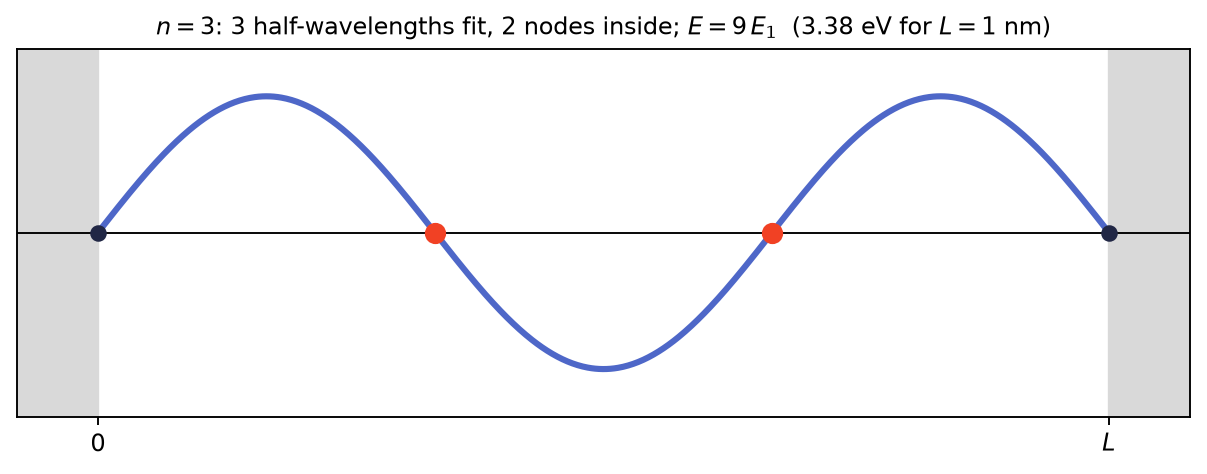
\includegraphics[width=\linewidth]{figures/box-1d.png}
\caption{The wave with $n=3$ half-wavelengths in a one-dimensional box.}
\end{figure}

\subsection{Two and three dimensions}

In a rectangular box with sides $L_x$ and $L_y$ the simplest waves that vanish on all walls are products, with a whole number per direction:
\[
\psi_{n_xn_y}=\sin\!\Big(\frac{n_x\pi x}{L_x}\Big)\sin\!\Big(\frac{n_y\pi y}{L_y}\Big),\qquad
E_{n_xn_y}=\frac{\pi^2\hbar^2}{2m_e}\Big(\frac{n_x^2}{L_x^2}+\frac{n_y^2}{L_y^2}\Big).
\]
The energies add because the kinetic energies of motion along $x$ and $y$ add. The wave changes sign across node lines: $n_x-1$ cross the $x$ direction and $n_y-1$ the $y$ direction. In three dimensions node lines become node planes and there are three whole numbers.

\begin{figure}[H]
\centering
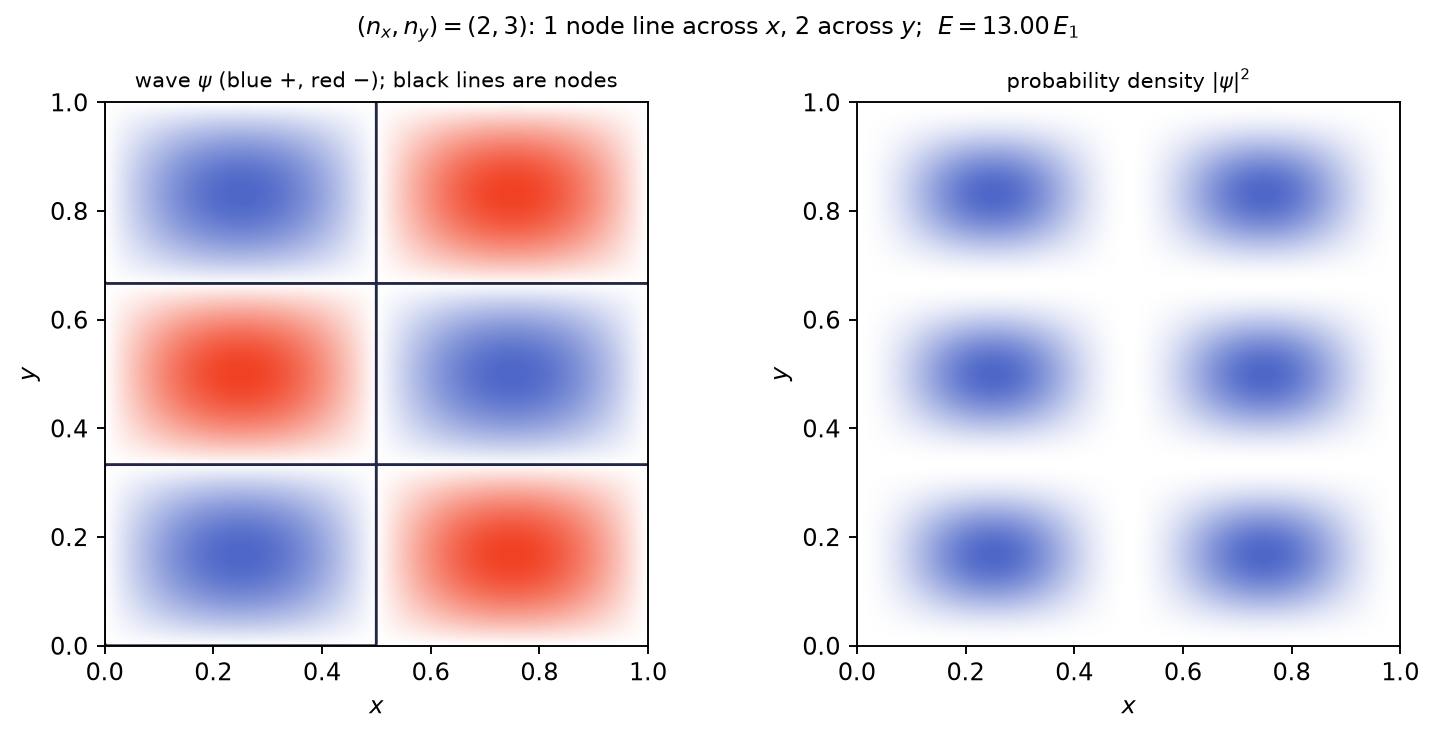
\includegraphics[width=0.75\linewidth]{figures/box-2d.png}
\caption{The wave with $(n_x,n_y)=(2,3)$ in a square box; blue is positive, red negative.}
\end{figure}

\subsection{The allowed waves form a lattice, and energy is a distance}

With $\mathbf k=(k_x,k_y)$, $k_x=n_x\pi/L_x$, $k_y=n_y\pi/L_y$, the energy is $E=\frac{\hbar^2}{2m_e}\lvert\mathbf k\rvert^2$. The allowed waves are the points of a rectangular grid in the $\mathbf k$-plane, and \emph{the energy of a state is the squared distance of its grid point from the corner}. The walls decide which grid points exist; the distance decides the energy.

\begin{figure}[H]
\centering
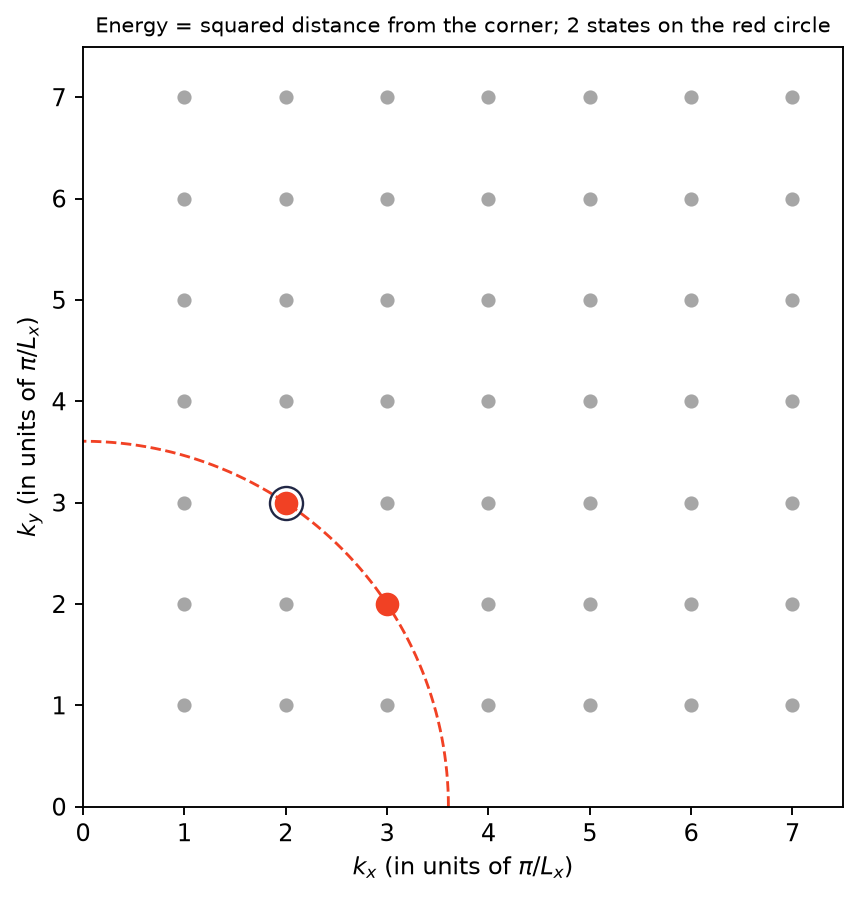
\includegraphics[width=\linewidth]{figures/box-kspace.png}
\caption{The allowed $\mathbf k$ values of a square box. States on one circle share an energy.}
\end{figure}

\subsection{Degeneracy is a sign of symmetry}

In a square box the states $(1,2)$ and $(2,1)$ are different waves with the same energy $5E_1$, because swapping $x$ and $y$ leaves the square unchanged. Some degeneracies have no such reason: $(1,7)$, $(5,5)$ and $(7,1)$ all have $50E_1$ because $1+49=25+25$ (an accidental degeneracy of whole numbers). Making one side longer removes the symmetry and splits the levels. In a cube the lowest levels have degeneracies $1,3,3,3,1,6$, most of them from permuting the three axes.

\begin{figure}[H]
\centering
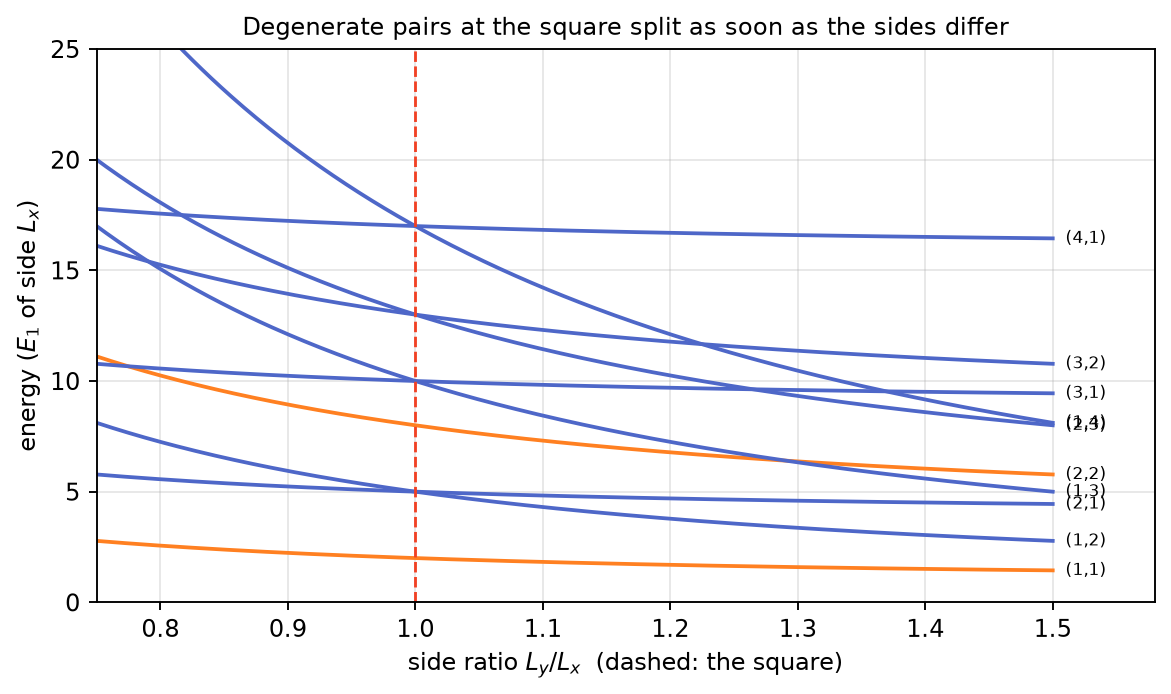
\includegraphics[width=0.75\linewidth]{figures/box-aspect-fan.png}
\caption{The lowest levels of a rectangular box as the ratio of the sides changes. At ratio 1 (the square) the symmetry gives degeneracies.}
\end{figure}

A sphere is the most symmetric container, and the degeneracy of the hydrogen levels ($n^2$ states in level $n$) follows from that.

\subsection{Counting states}

The number of states below $E$ is the number of grid points inside a quarter circle (2D) or one eighth of a sphere (3D); for large $E$ it is close to the area or volume. With $E$ in units of $E_1$,
\[
N_{1D}\approx\sqrt{E},\qquad N_{2D}\approx\frac{\pi}{4}E,\qquad N_{3D}\approx\frac{\pi}{6}E^{3/2}.
\]
More dimensions give many more states at the same energy, and the levels of a large box or a many-electron system merge into an almost continuous band. At atomic sizes the confinement energy is large: $E_1\propto1/L^2$ is tens of electronvolts for a box of about one bohr.

\begin{figure}[H]
\centering
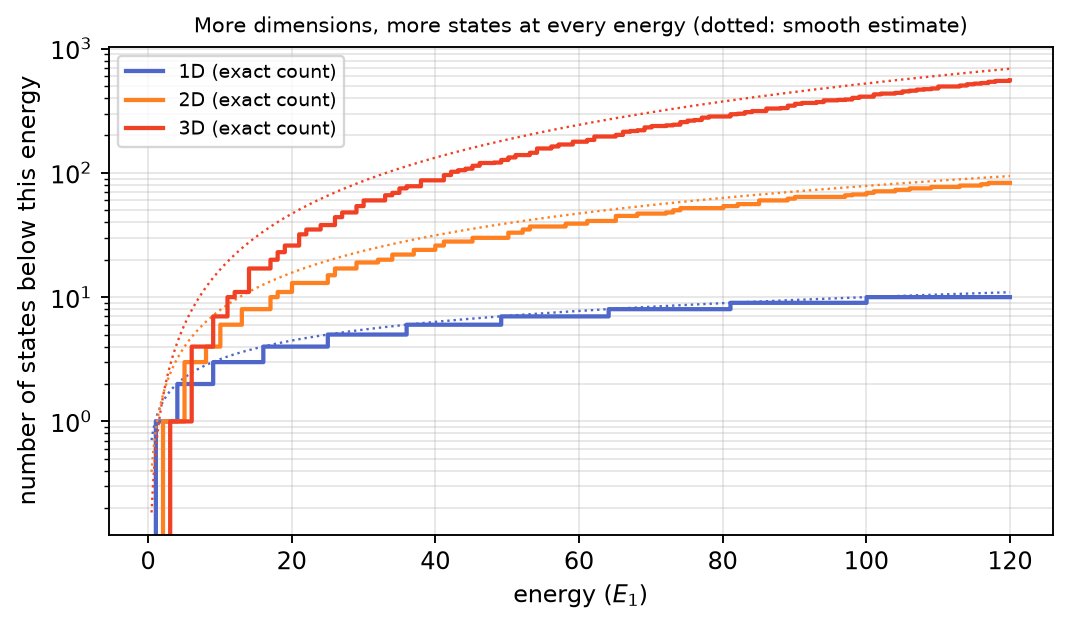
\includegraphics[width=0.75\linewidth]{figures/box-counting.png}
\caption{Number of states below an energy $E$ in one, two and three dimensions.}
\end{figure}

\paragraph{From a box to an atom.} An atom has no hard wall: the electron is held by the pull of the nucleus. Three things carry over: the wave must fit its surroundings (only some waves are allowed), each independent direction brings one whole number, and symmetry produces degeneracy. What changes is the choice of directions, which are no longer $x,y,z$ but distance $r$, polar angle $\vartheta$ and azimuth $\varphi$.

\paragraph{Further reading.} \cite{lt35,lt39}.

%%%%%%%%%%%%%%%%%%%%%%%%%%%%%%%%%%%%%%%%%%%%%%%%%%%%%%%%%%%%%%%%%%%%%%%%%%%%%%%%%%%%%%%%%%%%%%%%%%%%%%%%%%%%%%%%%%%%%%%%%%%%%%%%%%%%
%% HYDROGEN
%%%%%%%%%%%%%%%%%%%%%%%%%%%%%%%%%%%%%%%%%%%%%%%%%%%%%%%%%%%%%%%%%%%%%%%%%%%%%%%%%%%%%%%%%%%%%%%%%%%%%%%%%%%%%%%%%%%%%%%%%%%%%%%%%%%%

\section{Spheres and atoms: the hydrogen orbitals}\label{sec:hydrogen}

\noindent\emph{Notebook: \texttt{spherical\_harmonics\_and\_hydrogen.py}.}

\subsection{Spherical coordinates}

The natural coordinates for a potential that depends only on the distance from the nucleus are $r$, the polar angle $\vartheta$ (from the $z$ axis) and the azimuth $\varphi$ (around it). Volume elements change accordingly: $dV=dx\,dy\,dz$ becomes $r^2\sin\vartheta\,dr\,d\vartheta\,d\varphi$, and the Laplacian becomes
\[
\nabla^2=\partial_r^2+\frac2r\partial_r+\frac{\Lambda}{r^2},
\]
where $\Lambda$ contains only the angles. Because the potential depends on $r$ alone, the variables separate: $\psi(r,\vartheta,\varphi)=R(r)\,Y(\vartheta,\varphi)$.

\subsection{Nodes and direction}

In a box, node points, lines and planes cut across the coordinate axes. In spherical coordinates the three families of nodes are \emph{spheres} (constant $r$), \emph{cones} (constant $\vartheta$) and \emph{planes through the axis} (constant $\varphi$). Writing $n_r,n_\vartheta,n_\varphi$ for the number of nodes in each family, the angular nodes number $\ell=n_\vartheta+n_\varphi$, and the total number of nodes is $N_{\text{nodes}}=n-1=n_r+n_\vartheta+n_\varphi$. The shape of an orbital is the pattern of these nodes.

\subsection{Standing waves on a sphere}

The angular part satisfies the eigenvalue equation
\[
-\Lambda\,Y_{\ell m}=\ell(\ell+1)\,Y_{\ell m}.
\]
Single-valuedness and finiteness of a wave on a sphere force $m_\ell$ and $\ell$ to be whole numbers, with $\lvert m_\ell\rvert\le\ell$. The $2\ell+1$ functions with one $\ell$ share the angular energy $\ell(\ell+1)$ (degeneracy from the spherical symmetry). The functions $Y_{\ell m}$ are the \emph{spherical harmonics}; their real combinations give the familiar $s$, $p$, $d$ shapes, with $\lvert m_\ell\rvert$ nodal planes through the axis and $\ell-\lvert m_\ell\rvert$ nodal cones.

\begin{figure}[H]
\centering
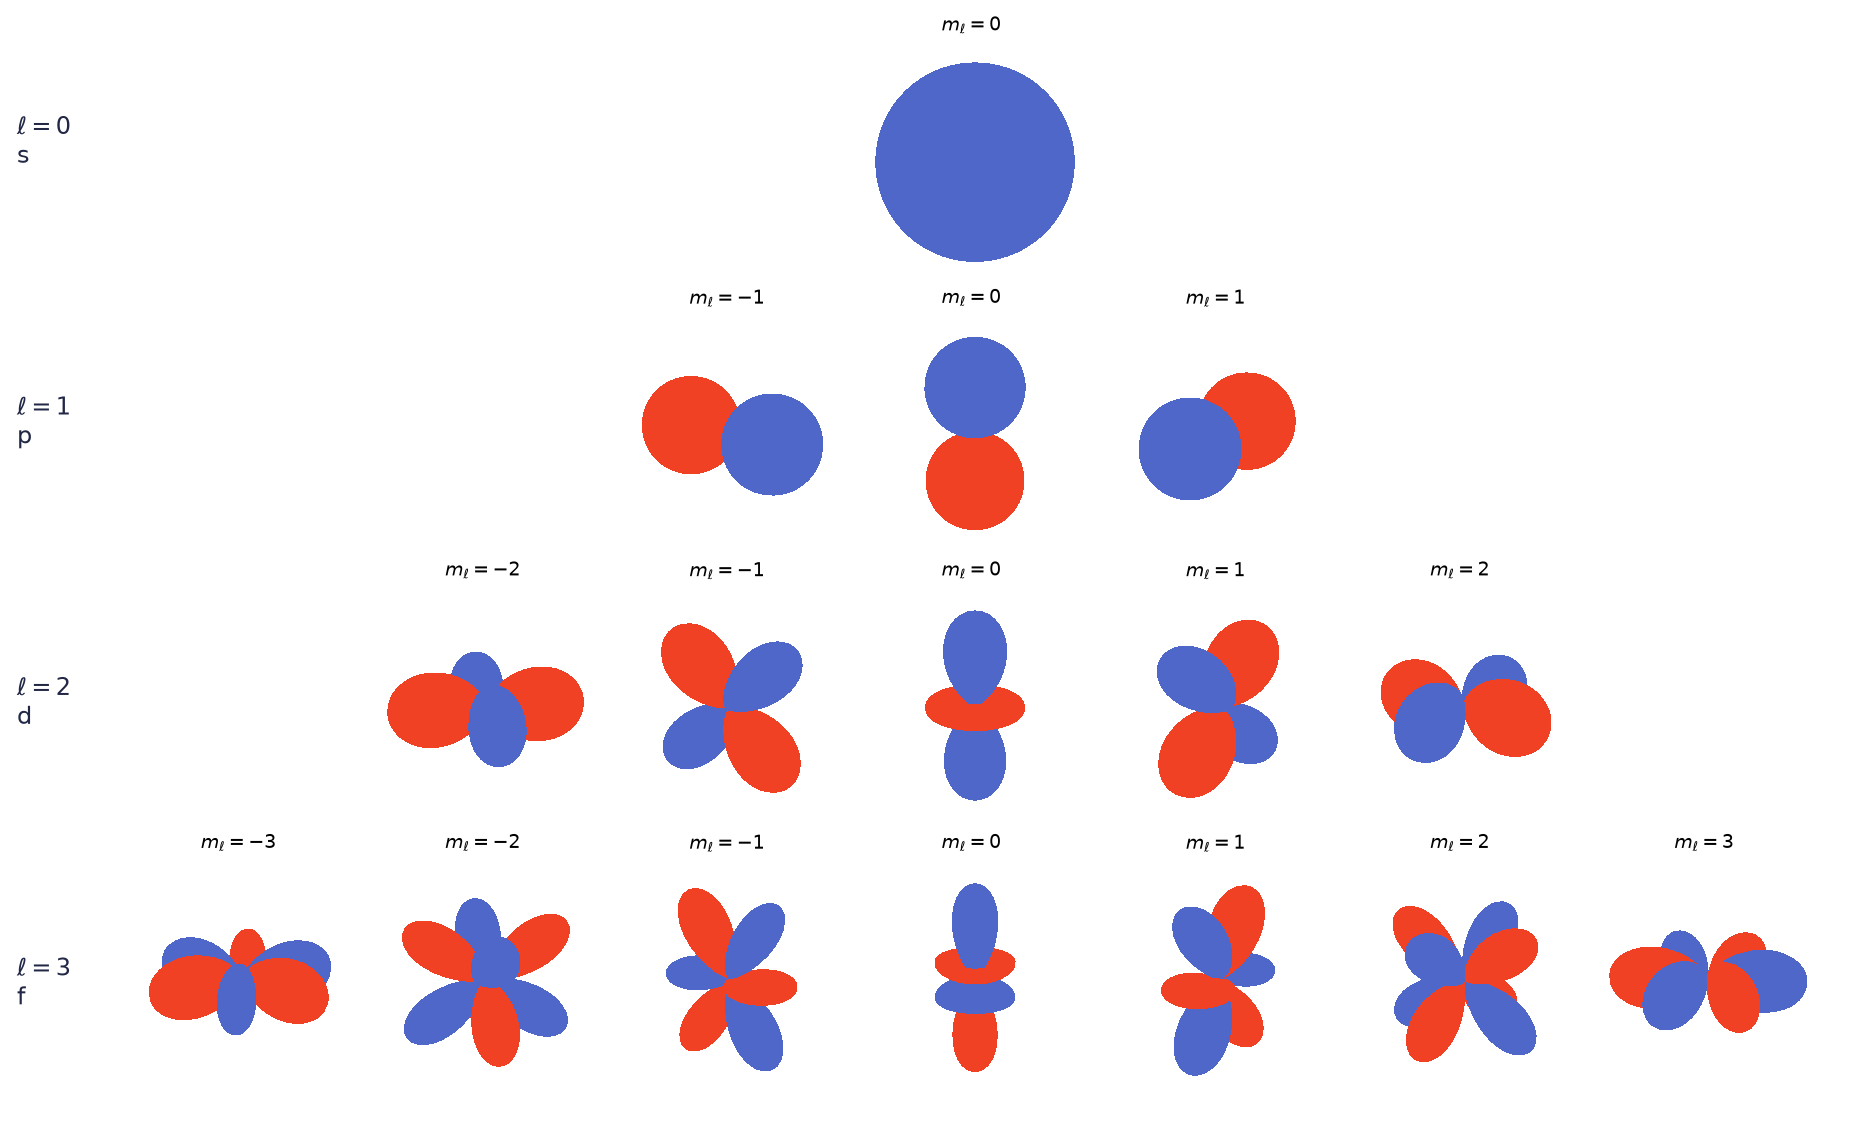
\includegraphics[width=\linewidth]{figures/harmonics-gallery.png}
\caption{Real spherical harmonics for $\ell=0$ to $3$.}
\end{figure}

\subsection{The radial part}

The radial equation for $u=rR$ has the same form as the angular one, an eigenvalue problem, with $\ell(\ell+1)$ entering as a fixed number:
\[
\Big[-\frac12\frac{d^2}{dr^2}+\underbrace{\frac{\ell(\ell+1)}{2r^2}+V(r)}_{V_{\text{eff}}}\Big]u=Eu .
\]
The term $\ell(\ell+1)/2r^2$ is a barrier that keeps waves with $\ell>0$ away from the nucleus. Each $\ell$ is therefore its own one-dimensional problem with its own ladder of energies, labelled by the number of radial nodes $n_r$. For hydrogen, $V=-1/r$, the energies are
\[
E_n=-\frac1{2n^2}\ \text{hartree}=-\frac{13.6}{n^2}\ \text{eV},\qquad n=n_r+\ell+1 .
\]
The energy depends on $n$ only, so level $n$ has $n^2$ orbitals ($2n^2$ with spin). That the energy does not depend on $\ell$ is special to the potential $-1/r$; the oscillator and the drumhead differ, and so does every atom with more than one electron (section \ref{sec:hf}).

\begin{figure}[H]
\centering
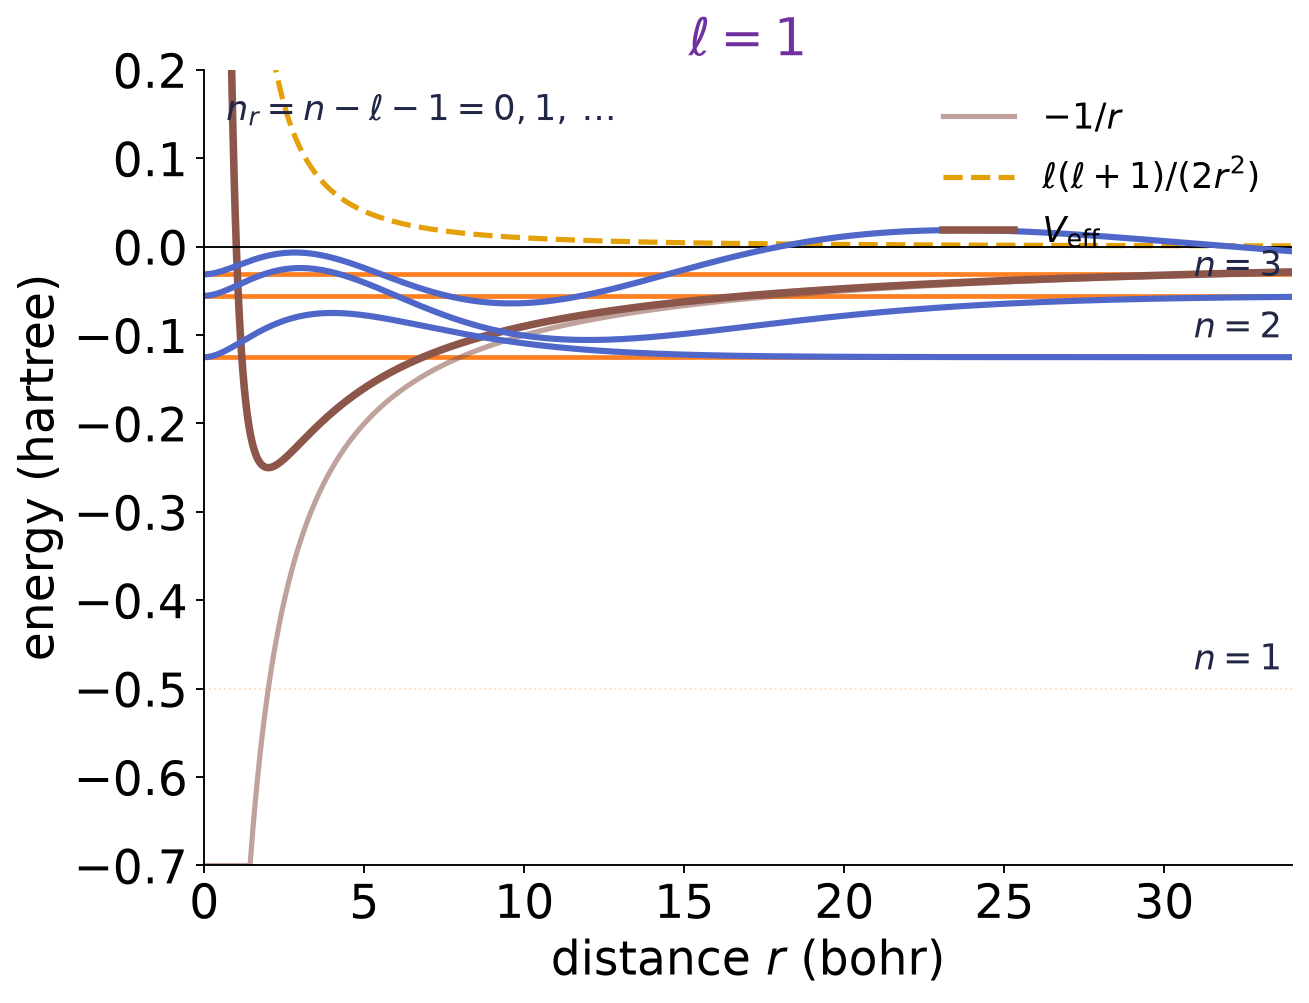
\includegraphics[width=\linewidth]{figures/hydrogen-central-levels.png}
\caption{The effective potential for $\ell=1$ (the barrier $\ell(\ell+1)/2r^2$ plus $-1/r$) and the lowest radial levels with their wave functions.}
\end{figure}

\subsection{Reading an orbital from its nodes}

The quantum numbers $(n_r,n_\vartheta,n_\varphi)$ say how many spheres, cones and planes the orbital has: a $3d$ orbital has $n=3$, $\ell=2$, so $N_{\text{nodes}}=2$ and no radial node; a $4f$ has $N_{\text{nodes}}=3$ and all three are angular. The energy counts $N_{\text{nodes}}$, the shape tells where they are.

\begin{figure}[H]
\centering
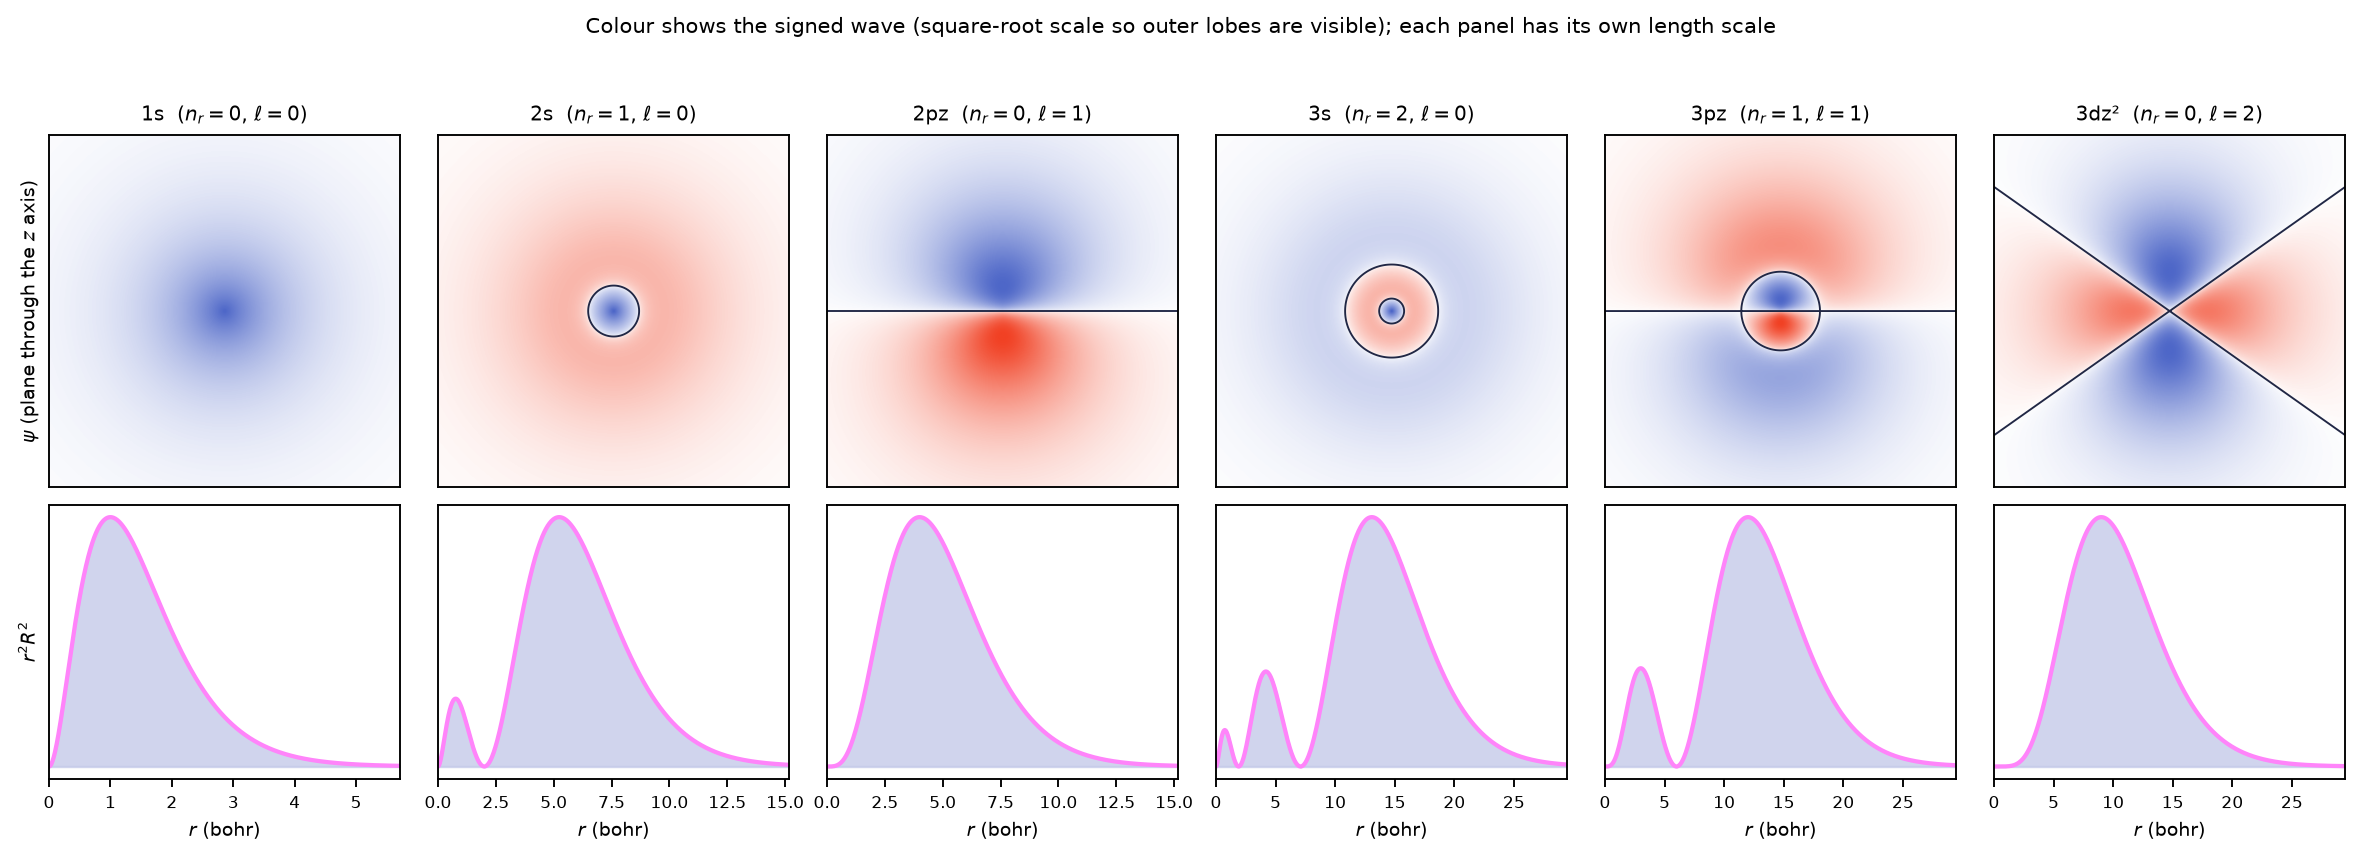
\includegraphics[width=\linewidth]{figures/hydrogen-orbital-gallery.png}
\caption{Sampled densities of hydrogen orbitals.}
\end{figure}

\paragraph{Further reading.} \cite{uc73,puc62,puc64,fowler,grinnell}.

%%%%%%%%%%%%%%%%%%%%%%%%%%%%%%%%%%%%%%%%%%%%%%%%%%%%%%%%%%%%%%%%%%%%%%%%%%%%%%%%%%%%%%%%%%%%%%%%%%%%%%%%%%%%%%%%%%%%%%%%%%%%%%%%%%%%
%% BRIDGE
%%%%%%%%%%%%%%%%%%%%%%%%%%%%%%%%%%%%%%%%%%%%%%%%%%%%%%%%%%%%%%%%%%%%%%%%%%%%%%%%%%%%%%%%%%%%%%%%%%%%%%%%%%%%%%%%%%%%%%%%%%%%%%%%%%%%

\section{From atoms to molecules: fixed nuclei, hybrids, methane}\label{sec:bridge}

\noindent\emph{Notebook: \texttt{from\_atoms\_to\_molecules.py}.}

Hydrogen is one of very few exactly solvable problems. A molecule has three complications: every particle adds three coordinates, the electrons push on each other through $1/\lvert\mathbf r_i-\mathbf r_j\rvert$, and there is no single centre of force. A table of the wave function on a grid with ten points per coordinate needs $10^N$ numbers for $N=3(N_{\text{nuclei}}+N_{\text{electrons}})$ coordinates: 45 coordinates for methane, 378 for caffeine. Three approximations, made one after the other, make a calculation possible: fixed nuclei, one orbital per electron (an orbital is a one-electron wave, two electrons of opposite spin to an orbital, each electron moving in the field of the nuclei and the average cloud of the others; section \ref{sec:hf}), and orbitals built from atom-centred functions (section \ref{sec:basis}). This section works out the first and shows the orbitals that the other two give: hybrids and the orbitals of methane.

\subsection{Fixed nuclei: Born--Oppenheimer}

A proton is 1836 times heavier than an electron, so the electrons settle into their lowest arrangement for each position of the nuclei. The approximation (1) freezes the nuclei at positions $\mathbf R$ and solves for the electrons, giving an energy $E_{\text{el}}(\mathbf R)$ that, with the nuclear repulsion, is a function of the nuclear positions only; and (2) uses that function as the potential for the much slower nuclear motion. The potential energy surface of every force field and geometry optimisation is this Born--Oppenheimer energy.

For H$_2^+$ (one electron, two protons a distance $R$ apart) the minimum of $E(R)$ is at $R\approx2.0$ bohr with a binding energy of about 2.8~eV. The nuclear problem is a one-dimensional standing-wave problem with reduced mass $\mu=M_p/2$,
\[
\Big[-\frac1{2\mu}\frac{d^2}{dR^2}+E(R)\Big]\chi(R)=E_{\text{tot}}\chi(R),
\]
whose levels have $0,1,2,\dots$ nodes. The two lowest are $0.010$~hartree ($0.27$~eV, about $2190\ \text{cm}^{-1}$) apart: about a tenth of the electron's binding energy, which is what ``the electrons are fast'' means in numbers. The spacing falls as $1/\sqrt{M}$, so lighter nuclei vibrate faster, and a heavier isotope changes the vibrational frequency but not the curve.

\begin{figure}[H]
\centering
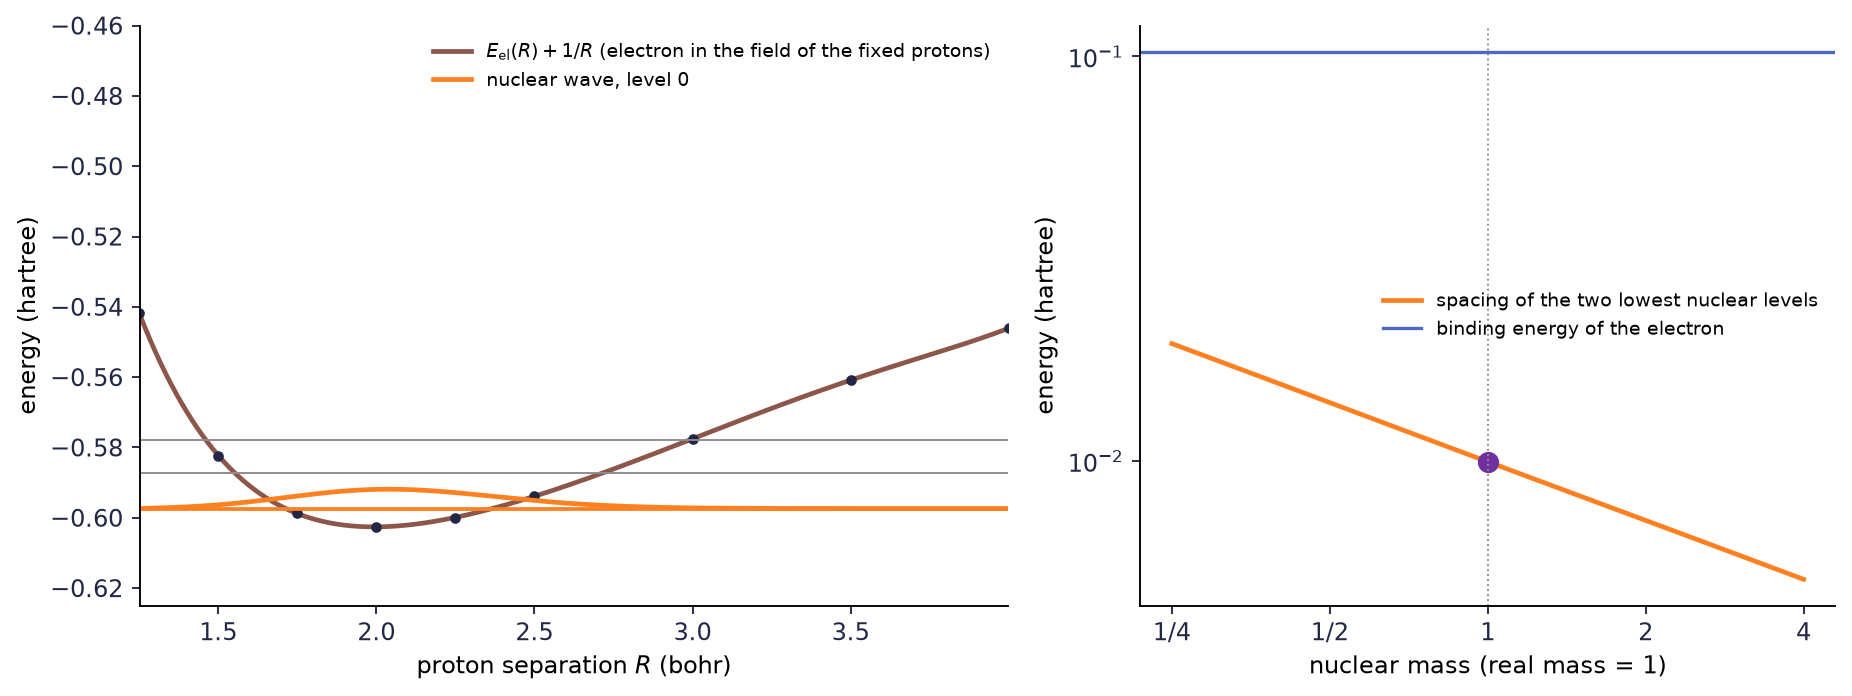
\includegraphics[width=\linewidth]{figures/bridge-born-oppenheimer.png}
\caption{H$_2^+$: the electronic energy as a potential for the nuclei, the lowest nuclear levels (left), and the level spacing against nuclear mass (right).}
\end{figure}

\subsection{Hybrid orbitals}

An atom in a molecule may use any mixture of its own $s$ and $p$ orbitals; the energy of the whole occupied set does not change. A useful family points one lobe in direction $\hat n$:
\[
h_{\hat n}=\frac{s+\sqrt n\,p_{\hat n}}{\sqrt{1+n}},\qquad n=1,2,3\ \text{for sp, sp}^2,\text{sp}^3 .
\]
Two such hybrids at angle $\theta$ overlap by $(1+n\cos\theta)/(1+n)$, and orbitals of one atom must be orthogonal, so
\[
1+n\cos\theta=0\ \Longrightarrow\ \theta=\arccos\!\big(-\tfrac1n\big)=180^\circ,\ 120^\circ,\ 109.47^\circ ,
\]
the angles of acetylene, ethene and methane. Four sp$^3$ hybrids $h_i=\tfrac12\big(s+\sqrt3\,\hat n_i\!\cdot\!\mathbf p\big)$, with $\hat n_i$ the corners of a tetrahedron, are orthonormal and each has one quarter $s$ character.

\begin{figure}[H]
\centering
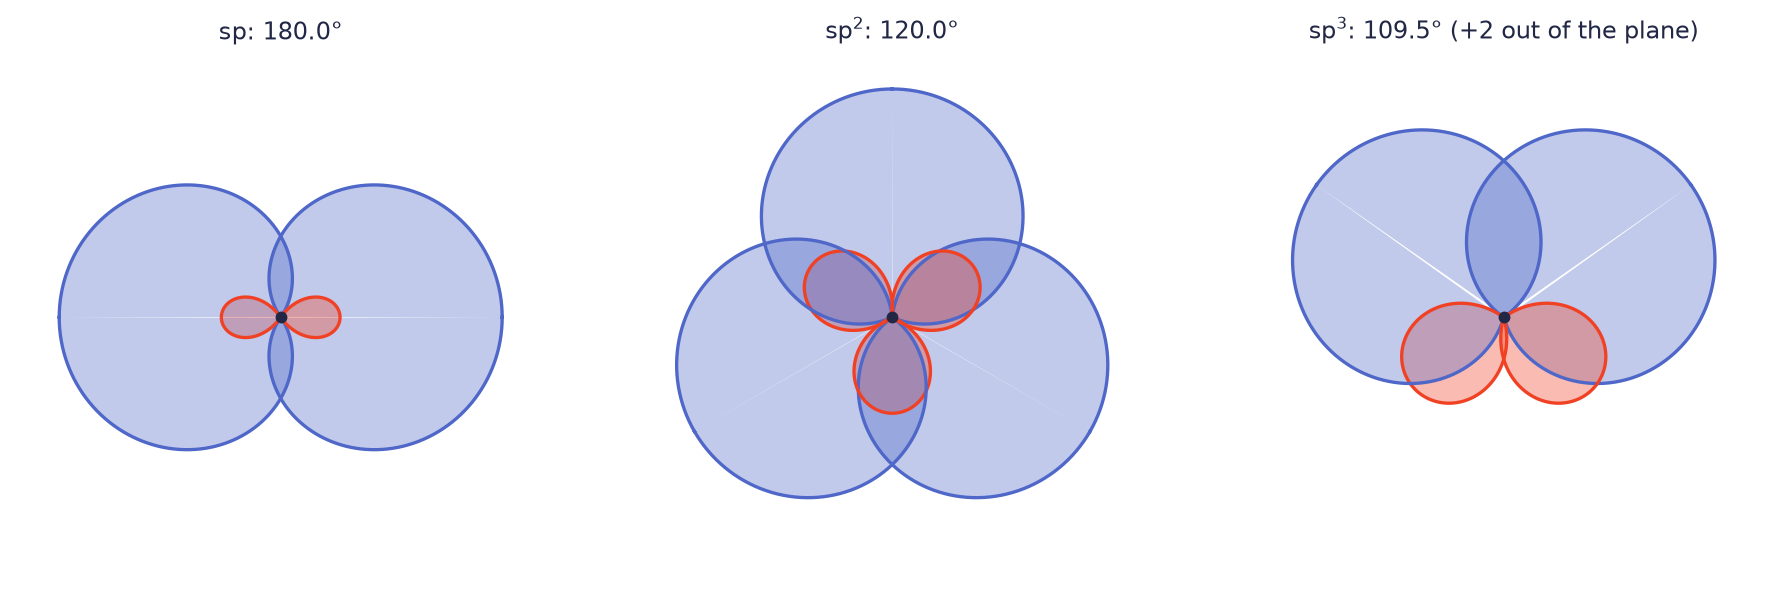
\includegraphics[width=\linewidth]{figures/bridge-hybrids.png}
\caption{Hybrids in the plane that holds them; blue positive, red negative.}
\end{figure}

\subsection{Methane: one level, then three}

Take as basis the carbon $2s$ and three $2p$ functions and one $1s$ function on each hydrogen: eight functions, eight molecular orbitals. Symmetry reduces the problem to $2\times2$ blocks: the carbon $2s$ couples only to the sum of the four $1s$ functions (one level of symmetry $a_1$), and each carbon $2p_i$ couples only to the hydrogen combination pointing the same way (three identical levels, $t_2$). The four lower levels are bonding (one $a_1$, three $t_2$) and the four upper ones antibonding; methane's eight valence electrons fill the bonding ones. A real calculation (wB97M-V/def2-TZVPD) gives the same pattern: occupied orbital energies $-10.319$ (carbon $1s$), $-0.813$ ($a_1$) and $-0.493$ hartree (three equal $t_2$).

The canonical orbitals are spread over the whole molecule. The four combinations $b_j=\tfrac12\big(a_1+\sqrt3\,\hat n_j\!\cdot\!\mathbf t_2\big)$ span exactly the same occupied space and so the same electron density, but each sits on one C--H bond: hybrids are a rewriting of the occupied orbitals, not a physical effect. On carbon the real bond orbital is $20\,\%$ $s$, $76\,\%$ $p$ and $4\,\%$ $d$, against $25:75:0$ for ideal sp$^3$: real bonds lie near the symmetric ideal.

\begin{figure}[H]
\centering
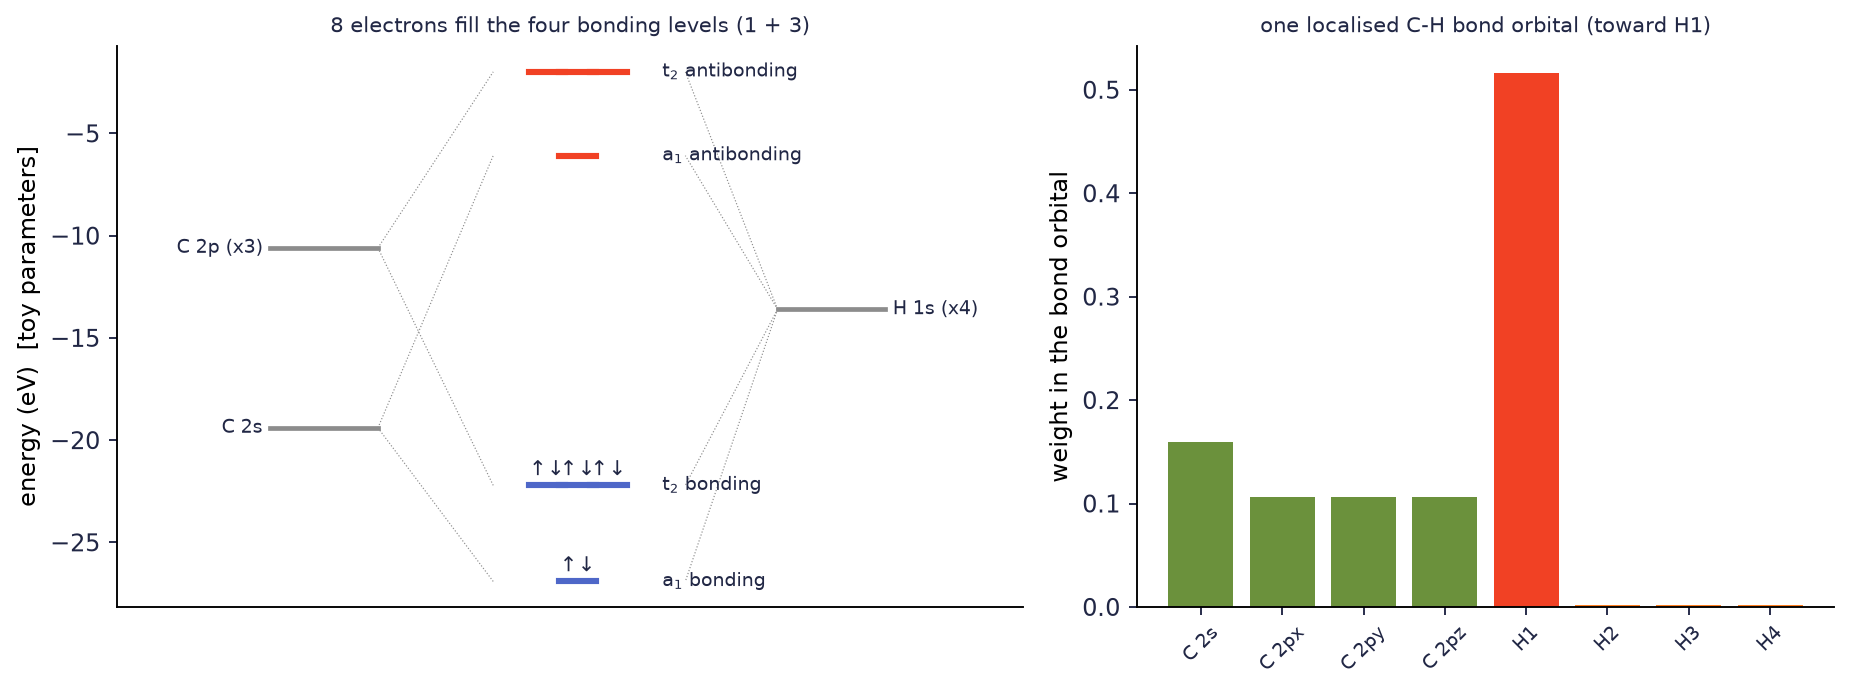
\includegraphics[width=\linewidth]{figures/bridge-methane.png}
\caption{A symmetry toy for methane (invented parameters; only the pattern is a result): its levels (left) and the weights of one localised bond orbital (right).}
\end{figure}

\paragraph{Further reading.} \cite{lt92,puc8,morsch,rioux,sherrillnotes}.

%%%%%%%%%%%%%%%%%%%%%%%%%%%%%%%%%%%%%%%%%%%%%%%%%%%%%%%%%%%%%%%%%%%%%%%%%%%%%%%%%%%%%%%%%%%%%%%%%%%%%%%%%%%%%%%%%%%%%%%%%%%%%%%%%%%%
%% BASIS SETS
%%%%%%%%%%%%%%%%%%%%%%%%%%%%%%%%%%%%%%%%%%%%%%%%%%%%%%%%%%%%%%%%%%%%%%%%%%%%%%%%%%%%%%%%%%%%%%%%%%%%%%%%%%%%%%%%%%%%%%%%%%%%%%%%%%%%

\section{Basis sets: from base states to \texttt{def2}}\label{sec:basis}

\noindent\emph{Notebook: \texttt{basis\_sets\_from\_base\_states.py}.}

\subsection{Base states, and what to do when they are unknown}

A stationary state $\psi_E$ solves $H\psi_E=E\psi_E$, and a general wave is a sum $\psi=\sum_nc_n\psi_{E_n}e^{-iE_nt/\hbar}$ of these base states. For hydrogen the base states are the orbitals of section \ref{sec:hydrogen}. For a molecule they are not known in closed form, so one builds the wave from other fixed functions $\chi_\nu$ that one is free to choose, $\psi=\sum_\nu c_\nu\chi_\nu$, and lets the coefficients adjust. Putting the sum into $H\psi=E\psi$, multiplying by $\chi_\mu$ and integrating gives a matrix equation,
\[
\sum_\nu H_{\mu\nu}c_\nu=E\sum_\nu S_{\mu\nu}c_\nu,\qquad
H_{\mu\nu}=\int\chi_\mu H\chi_\nu,\quad S_{\mu\nu}=\int\chi_\mu\chi_\nu ,
\]
which is the same as $\mathbf H\mathbf c=E\,\mathbf S\mathbf c$ (a generalized eigenproblem; $\mathbf S=\mathbf 1$ for orthonormal functions). The variational principle says that the lowest energy from a truncated sum is never below the exact one, and never rises when a function is added.

\subsection{Many nuclei: atom-centred functions (LCAO)}

For molecules the functions are centred on the atoms, $\psi=\sum_\mu c_\mu\chi_\mu$ (LCAO, linear combination of atomic orbitals), because an electron near a nucleus mostly feels that nucleus. For H$_2^+$, with one hydrogen $1s$ function $e^{-r}/\sqrt\pi$ on each proton, symmetry gives the bonding combination $c_A=c_B$ and the antibonding combination $c_A=-c_B$, with energies $E_\pm=(H_{AA}\pm H_{AB})/(1\pm S)$ plus the proton repulsion $1/R$. Only the bonding curve dips below the energy $-\frac12$ of a separated hydrogen atom and a proton. Two functions put the minimum at $R\approx2.49$ bohr with a binding energy of about 1.8~eV; a very large basis gives $R\approx2.0$ bohr and about 2.8~eV, so two functions give roughly 63\,\% of the bond energy and lie above the large-basis curve at every $R$, as the variational principle requires. Making the basis richer on each atom is what the rest of this section is about.

\begin{figure}[H]
\centering
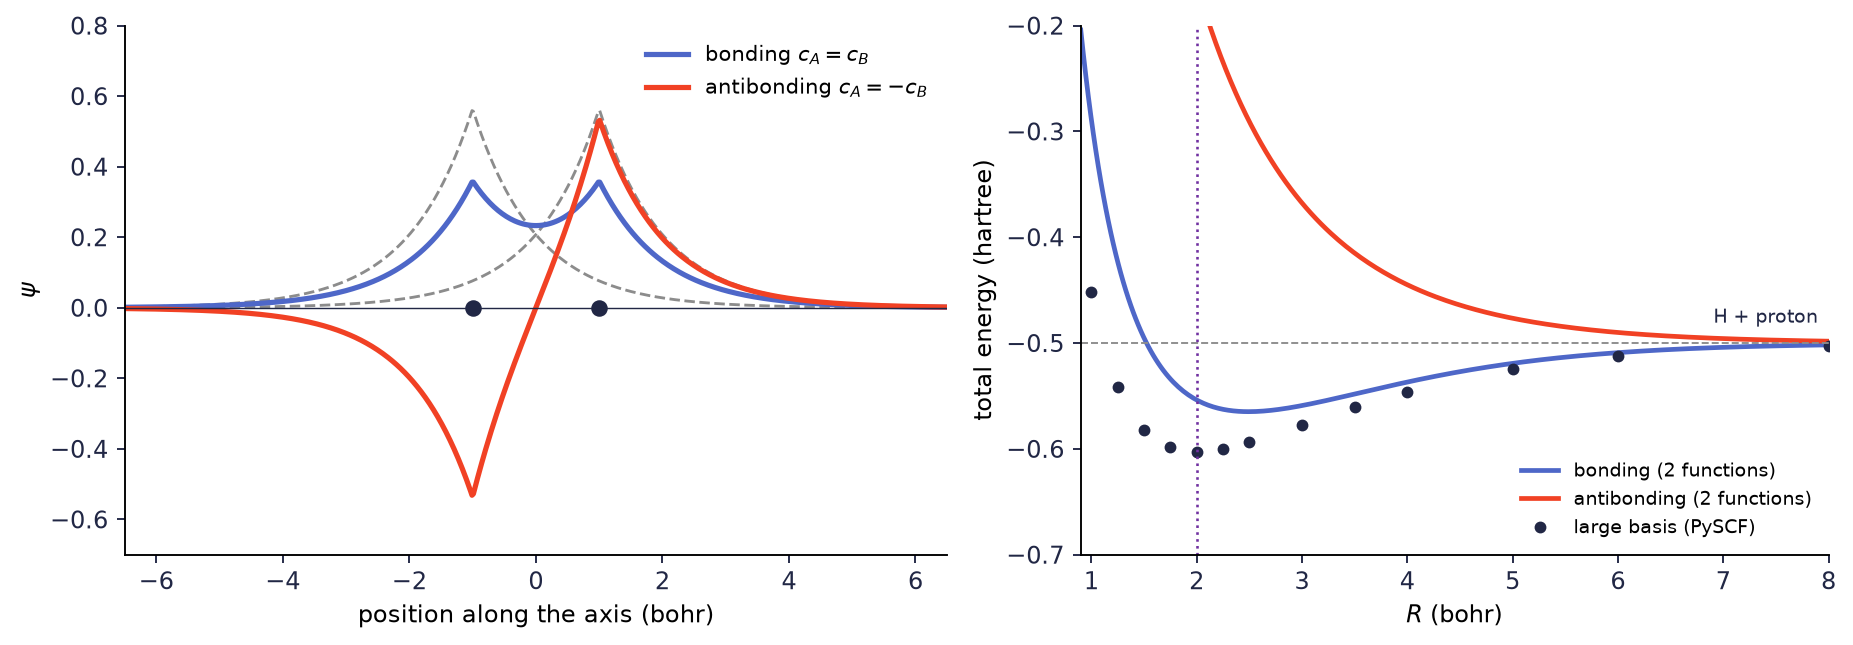
\includegraphics[width=\linewidth]{figures/basis-h2plus.png}
\caption{H$_2^+$ with one $1s$ function per proton: the bonding and antibonding combinations (left) and their energies, against a large-basis calculation (right).}
\end{figure}

\subsection{Slater and Gaussian functions}

The exact $1s$ function has a corner at the nucleus (the cusp, $\psi'(0)=-Z\psi(0)$) and a slow exponential tail, so a \emph{Slater-type} function $e^{-\zeta r}$ is a good copy. A \emph{Gaussian} $e^{-\alpha r^2}$ has neither: zero derivative at the centre and a tail that falls too fast. Gaussians are used anyway because the product of two Gaussians on different centres is a single Gaussian at a point between them,
\[
e^{-\alpha(x-A)^2}e^{-\beta(x-B)^2}=K\,e^{-(\alpha+\beta)(x-P)^2},\quad
P=\frac{\alpha A+\beta B}{\alpha+\beta},\quad K=e^{-\frac{\alpha\beta}{\alpha+\beta}(A-B)^2},
\]
so the millions of integrals in $\mathbf H$ and $\mathbf S$ are known in closed form and fast. The shape is repaired by \emph{contraction}: a fixed sum of $n$ Gaussians used as one function (STO-$n$G fits a Slater function by $n$ Gaussians).

\begin{figure}[H]
\centering
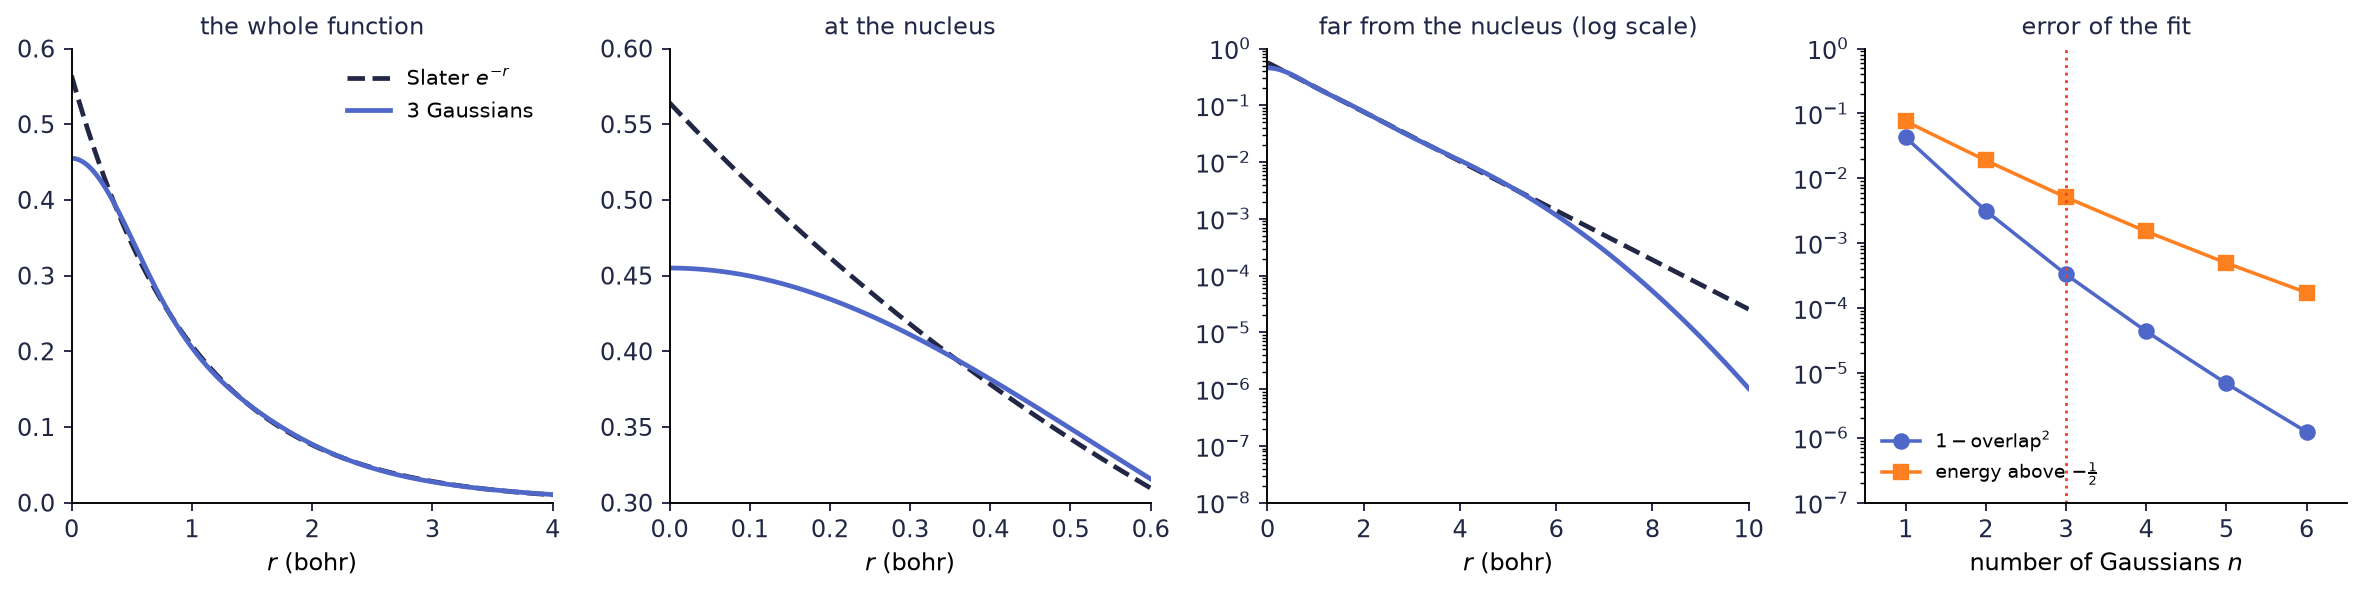
\includegraphics[width=\linewidth]{figures/basis-sto-fit.png}
\caption{A Slater $1s$ function and its fit by three Gaussians.}
\end{figure}

\subsection{Shells, zeta, polarization and diffuse functions}

A basis function is a radial part times a real spherical harmonic. A \emph{shell} of angular momentum $\ell$ is the set of $2\ell+1$ functions with one radial part: 1 for $s$, 3 for $p$, 5 for $d$, 7 for $f$. Several kinds of shells are combined:
\begin{itemize}
\item \textbf{Zeta} ($\zeta$): the valence shell is described by 2, 3 or 4 functions of different width (double, triple, quadruple zeta), so the orbital can swell or shrink in a bond.
\item \textbf{Polarization} (P): shells of higher angular momentum than the atom's occupied ones ($d$ on carbon, $p$ on hydrogen). Adding some $p_z$ to an $s$ function shifts the cloud off-centre, as a bond requires.
\item \textbf{Diffuse} (D): very wide, low-exponent functions for the far region, needed for anions, hydrogen bonds and dispersion.
\end{itemize}
In the label \texttt{def2-TZVPD}: \texttt{def2} is one consistent family of Gaussian basis sets (designed by Weigend and Ahlrichs), \texttt{TZ} is triple zeta, \texttt{V} says the extra functions are for the valence shells, \texttt{P} polarization, \texttt{D} diffuse. Water has 58 basis functions in \texttt{def2-TZVPD} and 74 in \texttt{def2-TZVPPD}, which differs only on hydrogen (one more $p$ shell and a $d$ shell).

\paragraph{Further reading.} \cite{sherrillbasis,hehre,bse,def2,bsse}.

%%%%%%%%%%%%%%%%%%%%%%%%%%%%%%%%%%%%%%%%%%%%%%%%%%%%%%%%%%%%%%%%%%%%%%%%%%%%%%%%%%%%%%%%%%%%%%%%%%%%%%%%%%%%%%%%%%%%%%%%%%%%%%%%%%%%
%% HARTREE-FOCK
%%%%%%%%%%%%%%%%%%%%%%%%%%%%%%%%%%%%%%%%%%%%%%%%%%%%%%%%%%%%%%%%%%%%%%%%%%%%%%%%%%%%%%%%%%%%%%%%%%%%%%%%%%%%%%%%%%%%%%%%%%%%%%%%%%%%

\section{Hartree--Fock: one orbital per electron in the field of the others}\label{sec:hf}

\noindent\emph{Notebook: \texttt{hartree\_fock\_mean\_field.py}.}

Orbitals are exact only for one-electron systems; for more electrons they are a construction, and Hartree--Fock finds the best ones. The order of this section follows Sherrill's introduction \cite{sherrillnotes}. The problem is the electronic Schr\"odinger equation at fixed nuclei, whose energy $E_{\text{el}}(\mathbf R)$ is the potential energy surface; everything difficult is in the electron repulsion $1/r_{12}$, which depends on two positions at once. If it were absent the problem would separate and the wave would be a product of one-electron functions, a \emph{Hartree product}. The orbital approximation keeps the product, gives each electron \emph{its own orbital} $\psi_i$ (a one-electron wave), and lets it feel the nuclei and the \emph{average} cloud of the others. This section shows where the average field comes from, writes it down, repairs the product's one symmetry defect, and explains the operator $\hat f$ that every later section uses.

\subsection{One orbital per electron: helium}

For helium, take both electrons in the hydrogen-like function $\varphi\propto e^{-\zeta r}$ (two electrons may share one spatial orbital only if their spins are opposite); the energy in hartree is
\[
E(\zeta)=\underbrace{\zeta^2}_{\text{kinetic}}\;\underbrace{-\,2Z\zeta}_{\text{attraction}}\;
{}+\underbrace{\tfrac58\zeta}_{\text{electron repulsion}},\qquad Z=2 .
\]
Without the repulsion the minimum is at $\zeta=2$ and $E=-4$. With it the minimum moves to $\zeta=Z-\tfrac5{16}=1.6875$, $E=-2.8477$ hartree: the repulsion acts as a \emph{screening}, and the orbital swells. The exact energy is $-2.9037$ and the best possible orbital product (the Hartree--Fock limit) is $-2.8617$.

\begin{figure}[H]
\centering
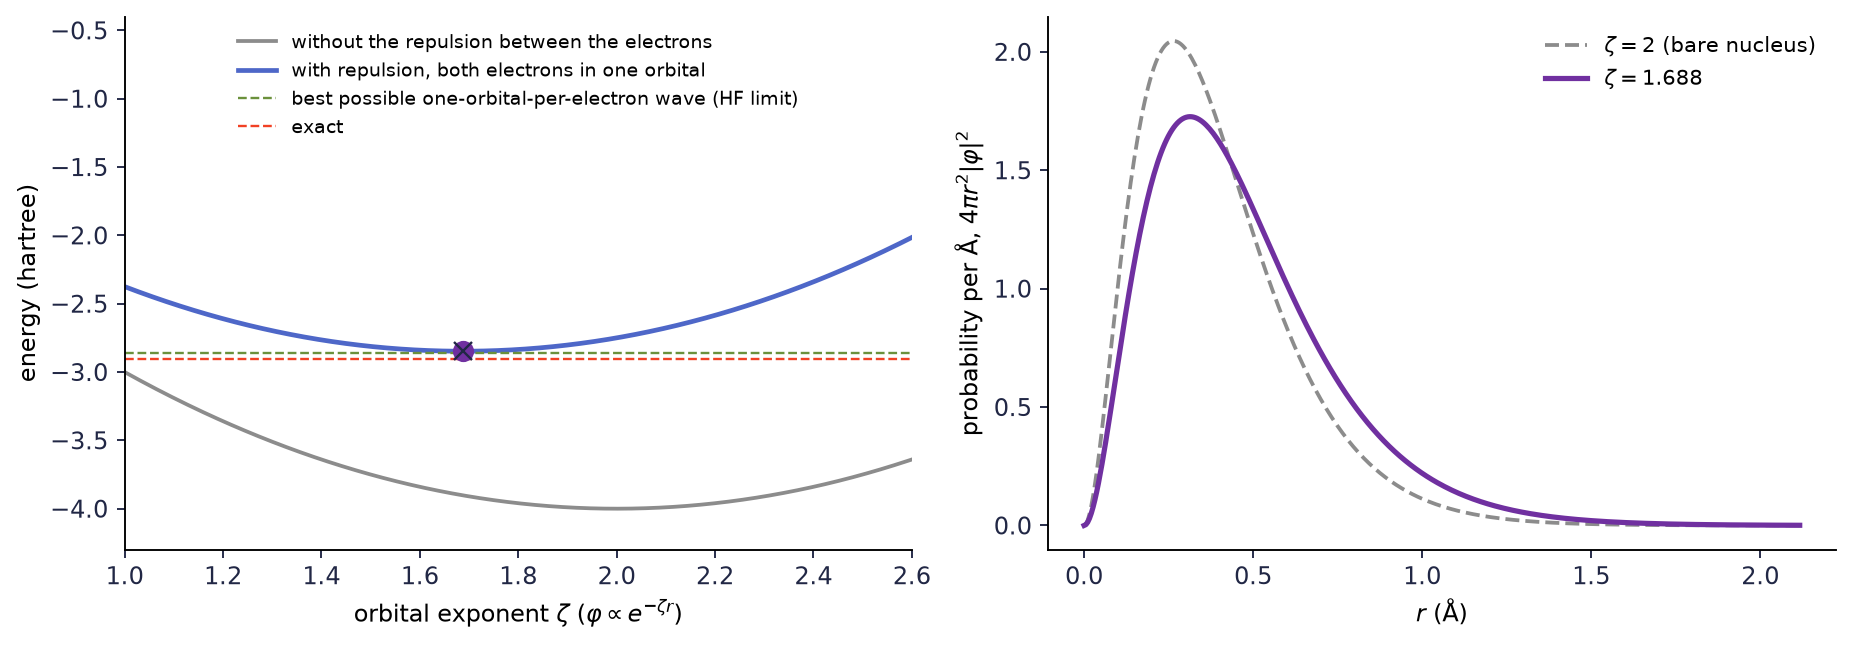
\includegraphics[width=\linewidth]{figures/bridge-helium.png}
\caption{Helium with one shared $1s$ orbital: energy against the orbital exponent $\zeta$ (left) and the radial density of the orbital (right).}
\end{figure}

\subsection{The average field of the other electrons}

In helium ``the average of the others'' is one electron, and $\tfrac58\zeta$ does not look like a field; it is one. Let the other electron have the density $\rho_{\text{other}}=\lvert\varphi\rvert^2$. An electron at $\mathbf r$ has the potential energy
\[
v_J(\mathbf r)=\int\frac{\rho_{\text{other}}(\mathbf r')}{\lvert\mathbf r-\mathbf r'\rvert}\,d\mathbf r',
\qquad
v_J(r)=\frac1r\Bigl[1-e^{-2\zeta r}(1+\zeta r)\Bigr]\ \text{ for }\varphi\propto e^{-\zeta r}.
\]
It tends to $1/r$ far away (the cloud looks like a point charge) and to the finite value $\zeta$ at $r=0$ (inside the cloud the charge outside cancels). The energy of one electron in this field is the average of $v_J$ over its own cloud, $\int\lvert\varphi\rvert^2v_J\,d\mathbf r=\tfrac58\zeta$: exactly the repulsion term of $E(\zeta)$. In lithium the two $1s$ electrons (exponent $\zeta_c=2.6875$) make the field $2v_J$, and the third electron sees the effective charge $Z_{\text{eff}}(r)=Z-2rv_J(r)=1+2e^{-2\zeta_cr}(1+\zeta_cr)$, which falls from $3$ at the nucleus to $1$ outside the core. The sum over all electrons in $v_J$ includes the electron's own cloud; the exchange term of the Fock operator removes this self-part.

\begin{figure}[H]
\centering
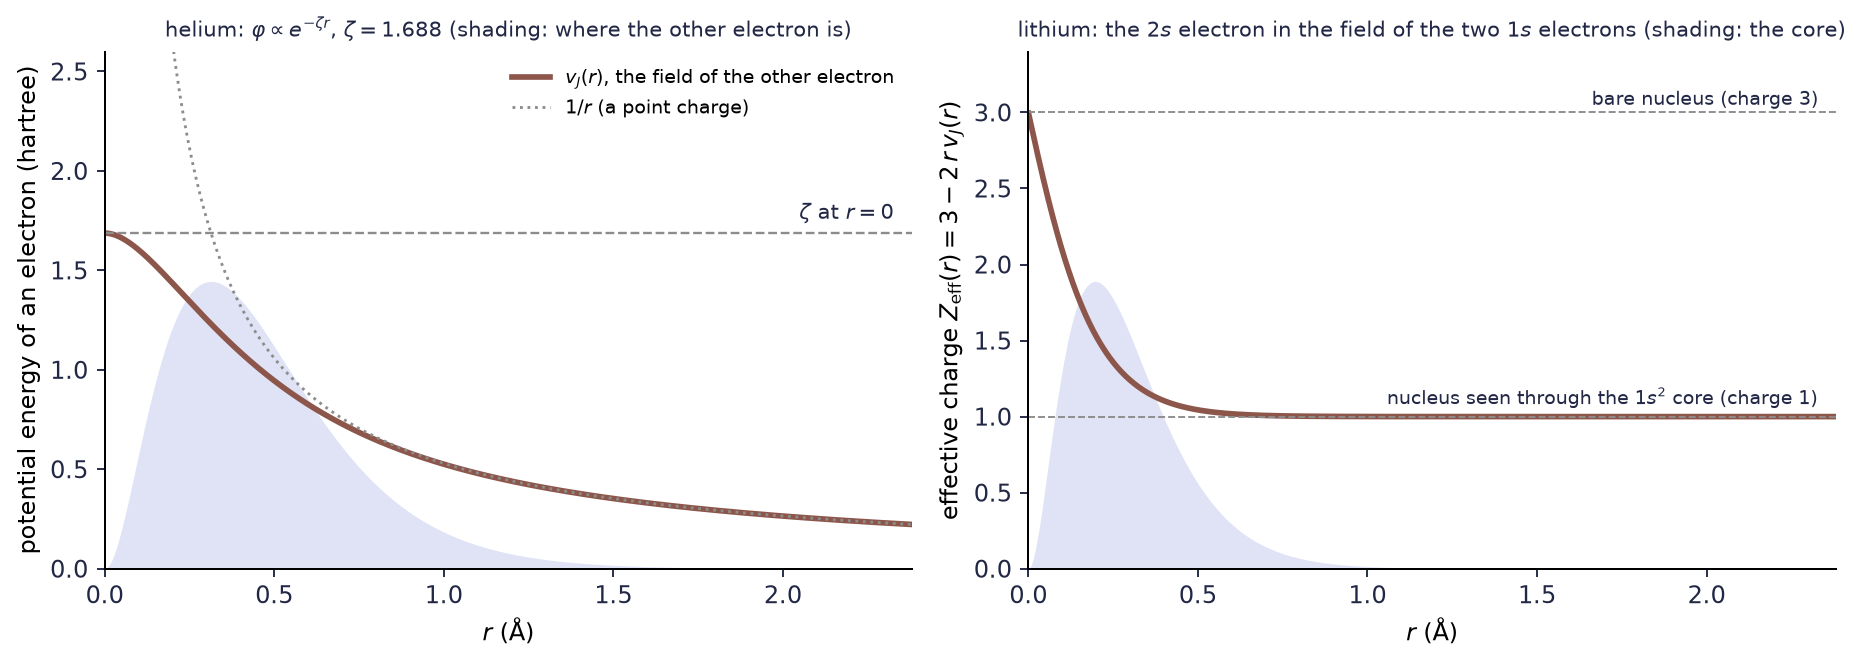
\includegraphics[width=\linewidth]{figures/hf-average-field.png}
\caption{Left: the field $v_J(r)$ of the other electron in helium, with the density that makes it (shading). Right: $Z_{\text{eff}}(r)$ of lithium.}
\end{figure}

\subsection{Screening: why $2s$ lies below $2p$}

In an atom with several electrons the potential seen by one electron is $-Z_{\text{eff}}(r)/r$, large close in and small far out. An $s$ wave is large near the nucleus and feels the strong pull there; a $p$ wave is kept away by the barrier $\ell(\ell+1)/2r^2$, feels the screened charge, and lies higher. In the toy with lithium's $Z_{\text{eff}}(r)$ and the core size $a=1/2\zeta_c$ as the one free parameter, the order is $s<p<d$ at each $n$, and the splitting grows with $a$; this is the origin of the familiar filling order. (The toy has one parameter, so only the ordering is a result.)

\begin{figure}[H]
\centering
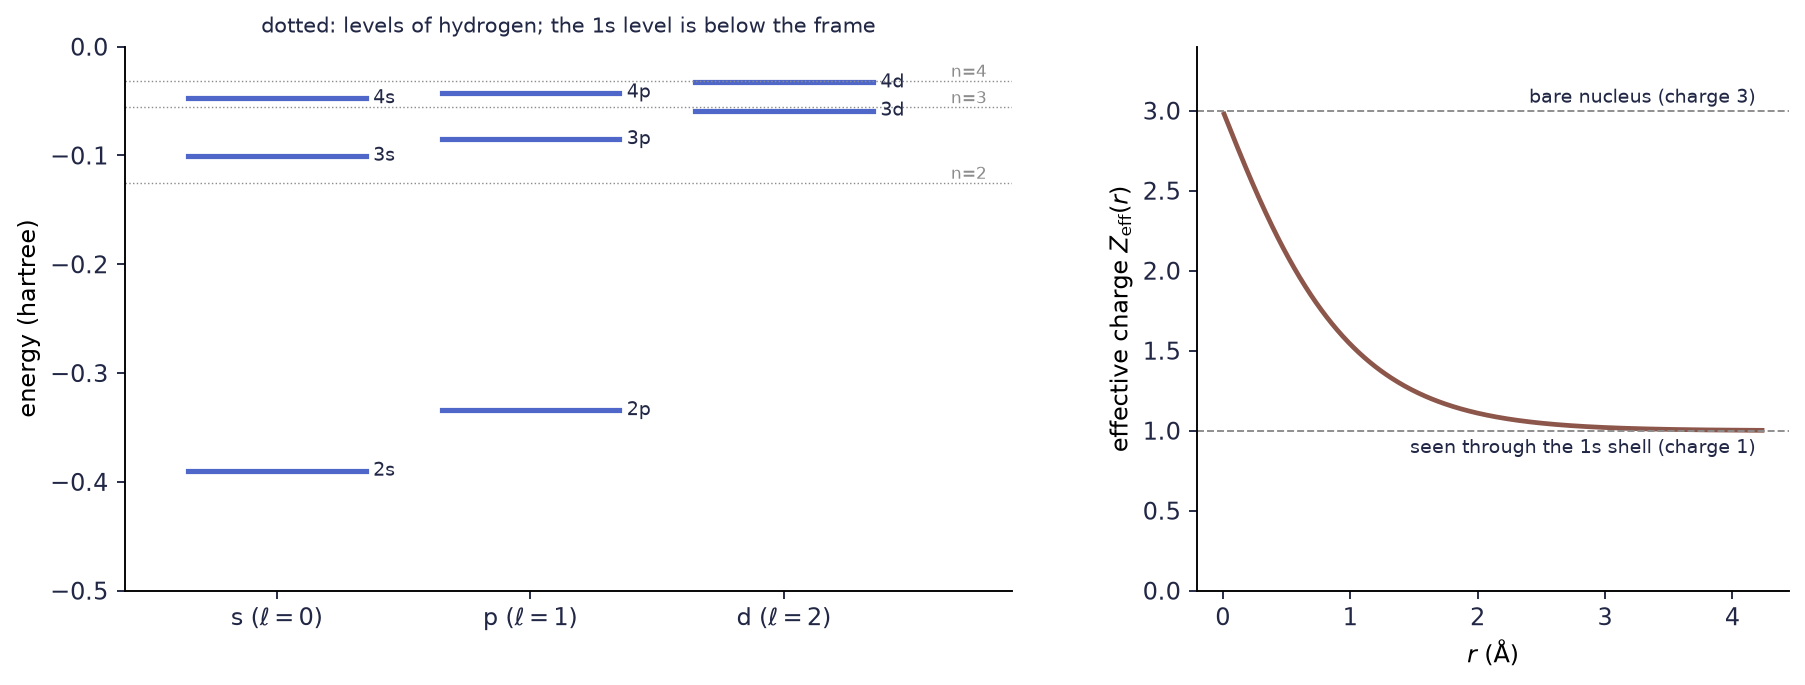
\includegraphics[width=\linewidth]{figures/bridge-screening.png}
\caption{Levels of the toy atom with a filled $1s$ shell (left) and its effective charge (right).}
\end{figure}

\subsection{Why the product fails: the Slater determinant}

Electrons also have a spin coordinate, and a spin orbital is a spatial orbital times $\alpha$ or $\beta$. Electrons are fermions: swapping the space-spin coordinates of two of them must flip the sign of $\Psi$ (the previous notes show where this comes from). A Hartree product does not do this, since $\psi_1(\mathbf x_2)\psi_2(\mathbf x_1)$ is in general not $-\psi_1(\mathbf x_1)\psi_2(\mathbf x_2)$, but a determinant does:
\[
\Psi(1,\dots,N)=\frac1{\sqrt{N!}}
\begin{vmatrix}
\psi_1(1)&\cdots&\psi_N(1)\\
\vdots&&\vdots\\
\psi_1(N)&\cdots&\psi_N(N)
\end{vmatrix}.
\]
Swapping two electrons swaps two rows, which flips the sign. Two electrons in the same orbital make two columns equal, so $\Psi=0$: the Pauli principle comes out for free. Each electron is associated with every orbital, so the electrons are indistinguishable. A single determinant is equivalent to each electron moving independently except for the Coulomb repulsion of the average positions of all electrons and an exchange interaction that keeps electrons of the same spin apart: Hartree--Fock is a mean-field model.

\subsection{The energy of a determinant}

Write the Hamiltonian with a one-electron operator $h=-\frac12\nabla^2-\sum_AZ_A/r_{iA}$ and a two-electron operator $v=1/r_{ij}$, so that $\hat H_{\text{el}}=\sum_ih(i)+\sum_{i<j}v(i,j)+V_{NN}$ with $V_{NN}$ constant. By the variational principle the best orbitals minimise $E=\langle\Psi|\hat H_{\text{el}}|\Psi\rangle$, and for a determinant this is
\[
E_{\text{HF}}=\sum_i\langle i|h|i\rangle+\tfrac12\sum_{i,j}\bigl(J_{ij}-K_{ij}\bigr),
\]
with the Coulomb integral $J_{ij}$ (repulsion of the charge clouds of orbitals $i$ and $j$) and the exchange integral $K_{ij}$ (the same with the two orbitals swapped, non-zero only for equal spins); the terms $i=j$ cancel. For helium, $J_{12}=\frac58\zeta$ and $K_{12}=0$ recover $E(\zeta)$.

\subsection{The Fock operator}

Minimising $E_{\text{HF}}$ with respect to the orbitals, which stay orthonormal (Lagrange multipliers), gives the Hartree--Fock equations
\[
\hat f\psi_i=\varepsilon_i\psi_i,\qquad \hat f=-\tfrac12\nabla^2+v_{\text{nuc}}+\hat J-\hat K .
\]
Here $\hat f$ is not an orbital: it is the \emph{one-electron effective Hamiltonian}, an operator that takes a function and returns another function. The equation is an eigenvalue equation; the orbitals $\psi_i$ are its eigenfunctions and the orbital energies $\varepsilon_i$ its eigenvalues. $-\frac12\nabla^2$ is the kinetic energy and $v_{\text{nuc}}$ the attraction to the nuclei. $\hat J$ is the average field of all the electrons, the $v_J$ above: $\hat J\psi_i=v_J\,\psi_i$. $\hat K$ is exchange, a correction for electrons of the same spin with no classical counterpart that comes entirely from antisymmetry; it mixes the other occupied orbitals into $\psi_i$, and its $j=i$ term cancels the self-repulsion contained in $\hat J$ (for one electron, $\hat J-\hat K=0$). The sum of the orbital energies counts every repulsion twice, so it is not the total energy. Because $\hat J$ and $\hat K$ are built from the occupied orbitals, $\hat f$ depends on its own solutions, which is why the equations are solved by iteration (below). Sherrill's $J_j$ and $K_j$ are the operators whose sums give our $\hat J$ and $\hat K$.

In a basis, $\psi_i=\sum_\mu C_{\mu i}\phi_\mu$, the equation becomes the matrix equation
\[
\mathbf F\mathbf C=\mathbf S\mathbf C\boldsymbol\varepsilon,\qquad F_{\mu\nu}=\int\phi_\mu\hat f\phi_\nu\,d\mathbf r,\quad S_{\mu\nu}=\int\phi_\mu\phi_\nu\,d\mathbf r,
\]
with $\mathbf F$ the Fock matrix and $\mathbf S$ the overlap matrix of the basis functions. Kohn--Sham DFT (next section) has the same form, with $\hat J-\hat K$ replaced by an effective potential: $\hat f=-\frac12\nabla^2+v_{\text{eff}}[\rho]$.

\subsection{The self-consistent loop}

At one set of nuclear positions: guess the orbitals (or the density), build $\hat f$ from them, solve $\hat f\psi_i=\varepsilon_i\psi_i$, form the new density from the occupied orbitals, and repeat until the density that built $\hat f$ and the density it gives agree.

\begin{figure}[H]
\centering
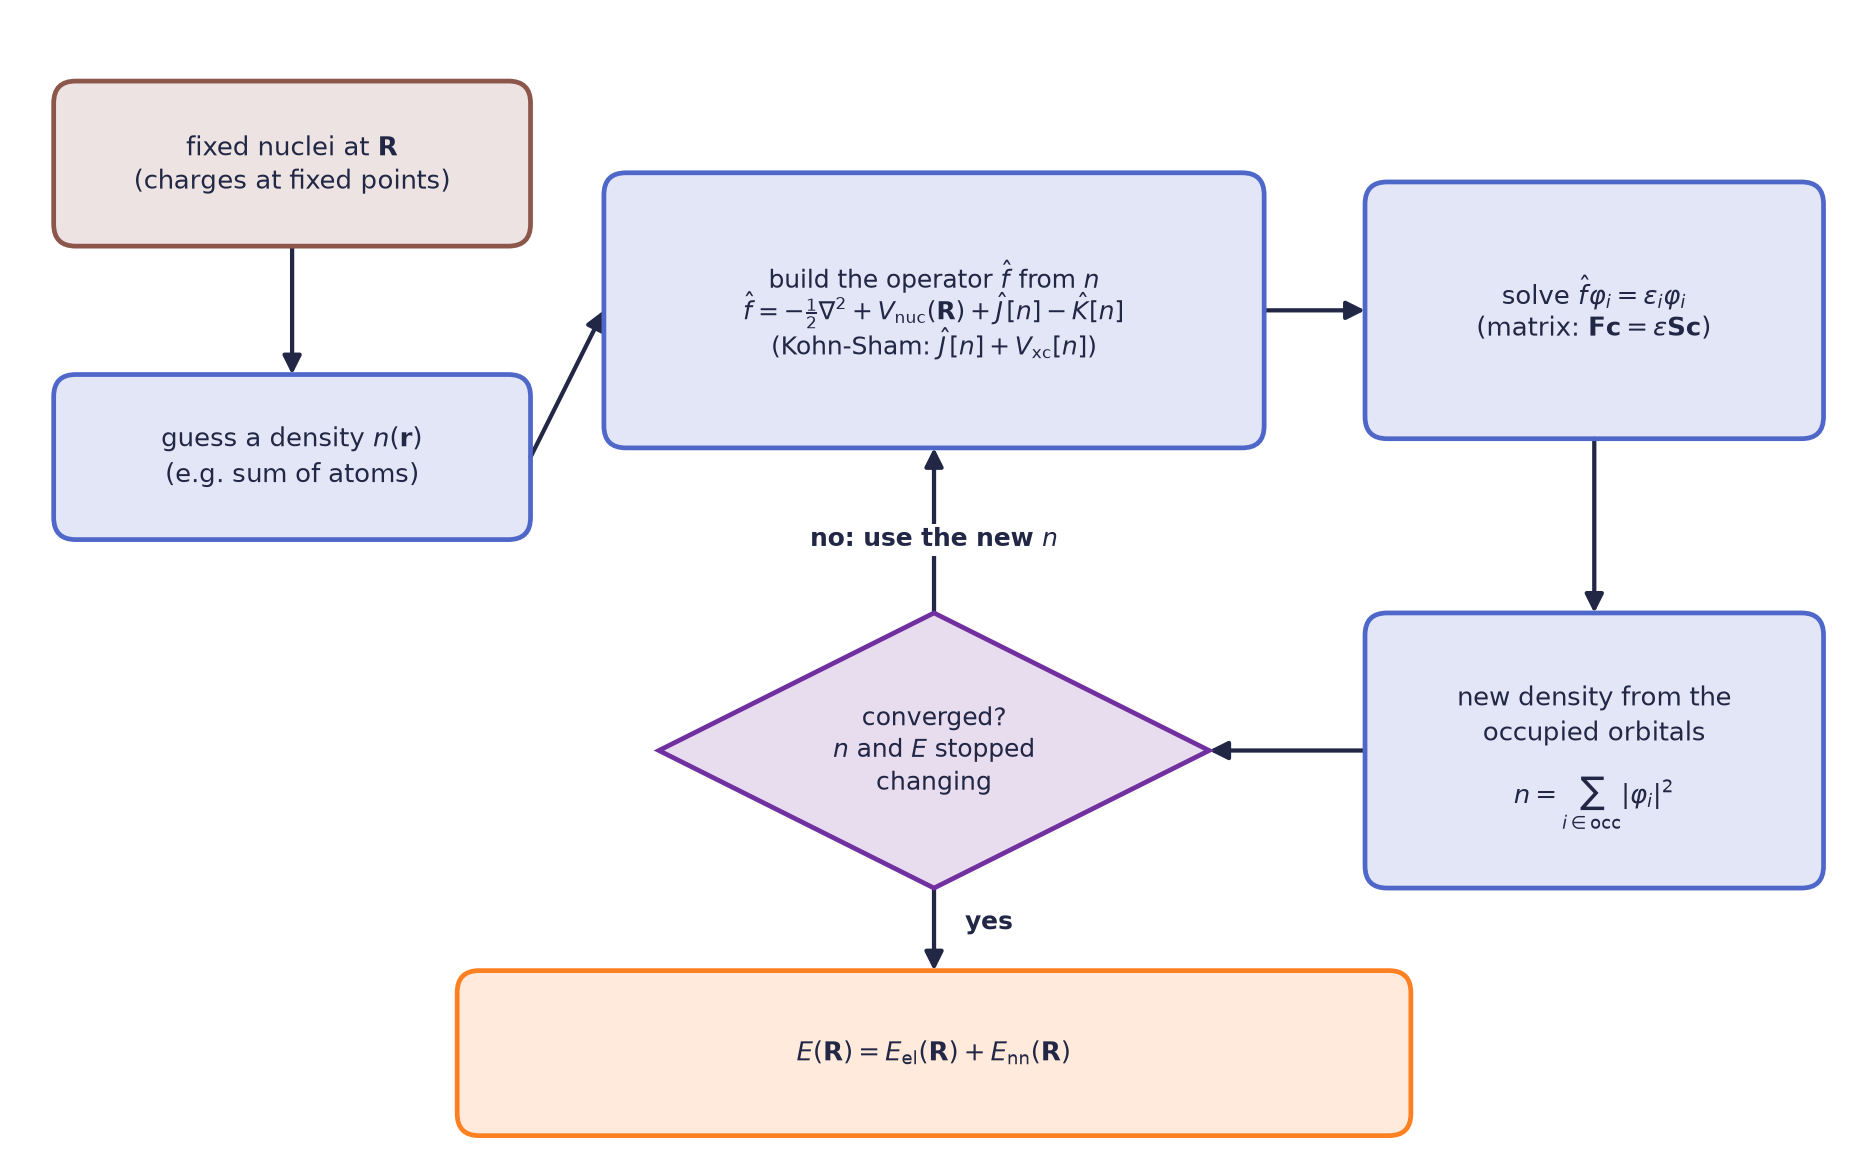
\includegraphics[width=0.9\linewidth]{figures/hf-scf-loop.png}
\caption{The self-consistent-field loop, the same for Hartree--Fock and Kohn--Sham.}
\end{figure}

\subsection{What Hartree--Fock misses}

Each electron sees only the \emph{average} position of the others; real electrons dodge each other, and the energy this saves is the correlation energy: $1.1$~eV in helium ($0.042$ hartree, 2\,\% of the energy). It is a small fraction of the total, but of the size of the energy differences chemistry cares about. Dispersion, the attraction between two uncharged molecules, is a pure correlation effect, so HF cannot produce it: HF finds two methane molecules repulsive. Two ways forward exist: wave-function methods (MP2, coupled cluster; section \ref{sec:cc}), accurate but with steeply rising cost, and density functional theory (next), with a cost close to HF's but an approximate exchange--correlation term.

\paragraph{Further reading.} \cite{sherrillnotes,puc8,psi4np}.

%%%%%%%%%%%%%%%%%%%%%%%%%%%%%%%%%%%%%%%%%%%%%%%%%%%%%%%%%%%%%%%%%%%%%%%%%%%%%%%%%%%%%%%%%%%%%%%%%%%%%%%%%%%%%%%%%%%%%%%%%%%%%%%%%%%%
%% DFT
%%%%%%%%%%%%%%%%%%%%%%%%%%%%%%%%%%%%%%%%%%%%%%%%%%%%%%%%%%%%%%%%%%%%%%%%%%%%%%%%%%%%%%%%%%%%%%%%%%%%%%%%%%%%%%%%%%%%%%%%%%%%%%%%%%%%

\section{Density functional theory and the Kohn--Sham matrix}\label{sec:dft}

\noindent\emph{Notebooks: \texttt{reading\_a\_dft\_label.py}, section 3, and \texttt{kohn\_sham\_matrix.py}.}

For $N$ electrons the wave function depends on $3N$ coordinates; DFT replaces it by the density $\rho(\mathbf r)$, which depends on three. The Hohenberg--Kohn theorem says the ground-state energy is determined by $\rho$ alone, so there is an energy functional $E[\rho]$. Nobody knows it exactly, but Kohn and Sham split it so that only a small piece is unknown: take non-interacting electrons that happen to have the same density as the real ones, with orbitals $\varphi_i$,
\[
\rho(\mathbf r)=\sum_i^{\text{occ}}\lvert\varphi_i(\mathbf r)\rvert^2,\qquad
E[\rho]=T_s[\rho]+E_{\text{nuc}}[\rho]+E_{\text{H}}[\rho]+E_{xc}[\rho].
\]
$T_s$ is the kinetic energy of the non-interacting electrons, $E_{\text{nuc}}$ the attraction to the nuclei, $E_{\text{H}}$ the classical repulsion of the density with itself, and $E_{xc}$ gathers everything left over (exchange and correlation). \emph{The ``functional'' in a DFT label is a specific approximation to $E_{xc}$}; everything else in the sum is exact.

\subsection{The matrix equation}

The orbitals satisfy $\hat f\psi_i=\varepsilon_i\psi_i$ with $\hat f=-\frac12\nabla^2+v_{\text{eff}}[\rho]$. Writing each orbital as a sum of $N$ fixed basis functions, $\psi_i=\sum_\mu C_{\mu i}\phi_\mu$, inserting it, multiplying by $\phi_\nu$ and integrating (as in section \ref{sec:basis}) gives
\[
\boxed{\,\mathbf F\mathbf C=\mathbf S\mathbf C\boldsymbol\varepsilon\,},\qquad
F_{\mu\nu}=\int\phi_\mu\hat f\phi_\nu\,d\mathbf r,\quad S_{\mu\nu}=\int\phi_\mu\phi_\nu\,d\mathbf r .
\]
Column $i$ of $\mathbf C$ holds the weights of orbital $i$, and $\boldsymbol\varepsilon$ is the diagonal matrix of orbital energies. $N$ basis functions give $N$ orbitals: for water in \texttt{def2-TZVPD}, 58 orbitals, of which the 5 lowest hold the 10 electrons and the other 53 are empty (virtual). Basis functions (indices $\mu,\nu$) are chosen before the calculation; orbitals (indices $i,j$) are its result.

\subsection{What is in $\mathbf F$}

\[
\mathbf F=\mathbf T+\mathbf V+\mathbf J[\mathbf D]+\mathbf V^{xc}[\mathbf D]+a\,\mathbf K[\mathbf D],
\]
where $\mathbf D=2\mathbf C_{\text{occ}}\mathbf C_{\text{occ}}^T$ is the density matrix. $\mathbf T$ (kinetic) and $\mathbf V$ (nuclear attraction) depend only on geometry and basis; $\mathbf J$ is the Coulomb repulsion of an electron with the whole density; $\mathbf V^{xc}$ is the exchange--correlation term, evaluated on a numerical grid; $a\mathbf K$ is the fraction $a$ of exact (Hartree--Fock) exchange that a hybrid functional mixes in ($a=0$ pure functional; $a=1$ with no $\mathbf V^{xc}$ is Hartree--Fock itself); and the ``-V'' in $\omega$B97M-V adds one more, non-local term. For the first element $F_{11}$ of water at $\omega$B97M-V/\texttt{def2-TZVPD} the pieces are (hartree) $T=+76.978$, $V=-99.580$, $J=+19.827$, $V^{xc}=-3.611$, VV10 $+0.005$ and exact exchange $-1.024$, adding up to $-7.404$. The big terms $T$, $V$ and $J$ nearly cancel; exchange--correlation is a small correction, which is why its approximation matters so much for energy \emph{differences}.

Everything except $\mathbf T$ and $\mathbf V$ depends on $\mathbf D$, which comes from solving with $\mathbf F$. That circularity is why the self-consistent-field (SCF) loop of section \ref{sec:hf} is repeated until the density stops changing.

\paragraph{Further reading.} \cite{kohn,burke,psi4np,pyscfdft}.

%%%%%%%%%%%%%%%%%%%%%%%%%%%%%%%%%%%%%%%%%%%%%%%%%%%%%%%%%%%%%%%%%%%%%%%%%%%%%%%%%%%%%%%%%%%%%%%%%%%%%%%%%%%%%%%%%%%%%%%%%%%%%%%%%%%%
%% LABEL
%%%%%%%%%%%%%%%%%%%%%%%%%%%%%%%%%%%%%%%%%%%%%%%%%%%%%%%%%%%%%%%%%%%%%%%%%%%%%%%%%%%%%%%%%%%%%%%%%%%%%%%%%%%%%%%%%%%%%%%%%%%%%%%%%%%%

\section{Reading a DFT label}\label{sec:label}

\noindent\emph{Notebook: \texttt{reading\_a\_dft\_label.py}.}

The two labels of the machine-learning datasets used in the lab are
\begin{center}
\begin{tabular}{lll}
\hline
 & OMol25 & SPICE II \\
\hline
Functional & $\omega$B97M-V & $\omega$B97M \\
Dispersion & part of the functional (VV10) & added afterwards (D3 with BJ damping) \\
Basis set & \texttt{def2-TZVPD} & \texttt{def2-TZVPPD} \\
Written as & $\omega$B97M-V/\texttt{def2-TZVPD} & $\omega$B97M-D3(BJ)/\texttt{def2-TZVPPD} \\
\hline
\end{tabular}
\end{center}
Three choices define the level of theory: the \textbf{functional} (how the electron interaction is approximated), the \textbf{dispersion treatment} (how the weak attraction between neighbouring molecules is described) and the \textbf{basis set} (what shapes the orbitals are built from). Underneath are settings that are usually \emph{not} in the label but still change the number: the integration grid, the convergence thresholds and the program.

\subsection{The basis set and why the D matters}

When two molecules are close, each can ``borrow'' the other's basis functions to describe its own electrons better, and the energy drops for a reason unrelated to chemistry: the basis-set superposition error (BSSE). The \emph{counterpoise} correction recomputes each monomer in the full dimer basis, using ghost atoms (basis functions without nuclei or electrons). A molecule gains energy by borrowing only if its own basis is missing something: the faint tail of its cloud that reaches toward the neighbour. A diffuse function is still centred on its own atom, but its small exponent lets it describe that tail, so there is nothing left to borrow. Most of the drop in BSSE from \texttt{def2-TZVP} to \texttt{def2-TZVPD} is exactly this. Anions need diffuse functions for the same reason: the extra electron is loosely bound.

\begin{figure}[H]
\centering
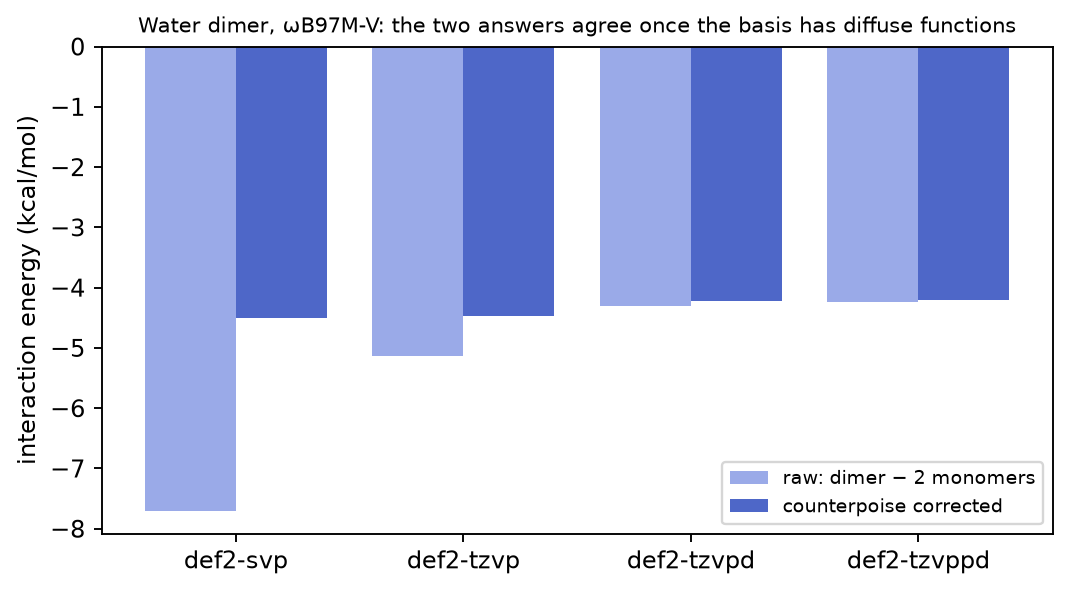
\includegraphics[width=\linewidth]{figures/dft-bsse.png}
\caption{Water dimer at $\omega$B97M-V: interaction energy with and without the counterpoise correction, for several basis sets.}
\end{figure}

\subsection{The functional: Jacob's ladder}

Approximations to $E_{xc}$ can be sorted by what they are allowed to look at, as the rungs of a ladder:
\begin{center}
\begin{tabular}{lll}
\hline
Rung & Looks at & Examples \\
\hline
1. LDA & the density $\rho$ at each point & SVWN \\
2. GGA & $\rho$ and its gradient $\lvert\nabla\rho\rvert$ & PBE, B97 \\
3. meta-GGA & also the kinetic energy density $\tau$ & r2SCAN, $\omega$B97M (the M) \\
4. hybrid & also some exact (HF) exchange from the orbitals & B3LYP, $\omega$B97X, $\omega$B97M \\
5. double hybrid & also virtual orbitals & (not used for these datasets) \\
\hline
\end{tabular}
\end{center}
\textbf{B97} names the form of the GGA part: Becke's 1997 functional writes exchange and correlation as power series in the reduced gradient with fitted coefficients, and the members of the family (B97, $\omega$B97, $\omega$B97X, $\omega$B97X-V, $\omega$B97M-V) share a shape and differ in how the coefficients were chosen. \textbf{M} means meta: the functional also uses $\tau(\mathbf r)=\frac12\sum_i\lvert\nabla\varphi_i\rvert^2$. Compared with its value $\tau_W$ for a single orbital, $\tau$ tells the functional what kind of region it is in: $\tau\approx\tau_W$ where one orbital dominates (far outside the molecule, in the oxygen $1s$ core), $\tau>\tau_W$ where several overlap (the bonding region). A GGA cannot make this distinction; a meta-GGA can.

\begin{figure}[H]
\centering
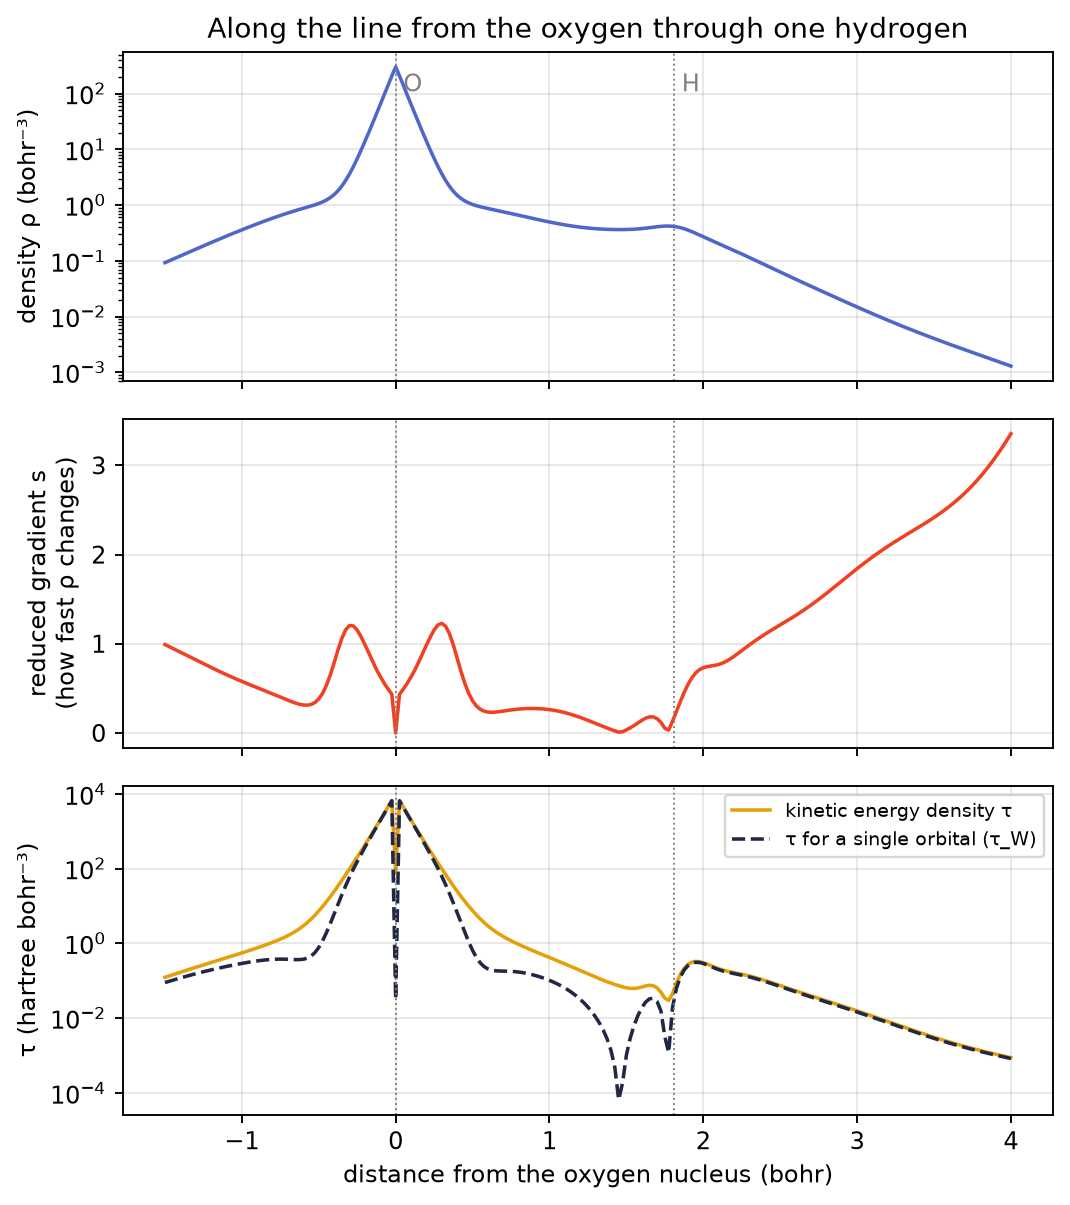
\includegraphics[width=\linewidth]{figures/dft-line-fields.png}
\caption{The ingredients a functional looks at, on a line from the oxygen nucleus through one hydrogen of water.}
\end{figure}

\subsection{Exact exchange and range separation: $\omega$}

Exchange between electrons of the same spin is known exactly from Hartree--Fock theory; in DFT it is approximated, with a known flaw: an electron partly repels itself (self-interaction error). Mixing in some exact exchange gives a hybrid (B3LYP uses 20\,\% everywhere). A \emph{range-separated} hybrid is smarter about where: it splits the repulsion in two,
\[
\frac1r=\underbrace{\frac{\operatorname{erfc}(\omega r)}{r}}_{\text{short range}}+\underbrace{\frac{\operatorname{erf}(\omega r)}{r}}_{\text{long range}},
\]
where $\omega$ is the splitting parameter (unrelated to angular frequency) and $r$ the distance between two electrons. Up close the density functional does the job; far away the exact $1/r$ tail matters, so the long-range part uses 100\,\% exact exchange. For $\omega$B97M-V, $\omega=0.3$~bohr$^{-1}$ with 100\,\% long-range and 15\,\% short-range exact exchange. A test of why this matters: for the exact functional the energy of the highest occupied orbital equals minus the ionisation energy. Local functionals and B3LYP miss by 3 to 5~eV, because their wrong tail lets the outermost electron drift away too easily; range-separated hybrids land within about 1~eV (the experimental value for water is 12.6~eV).

\begin{figure}[H]
\centering
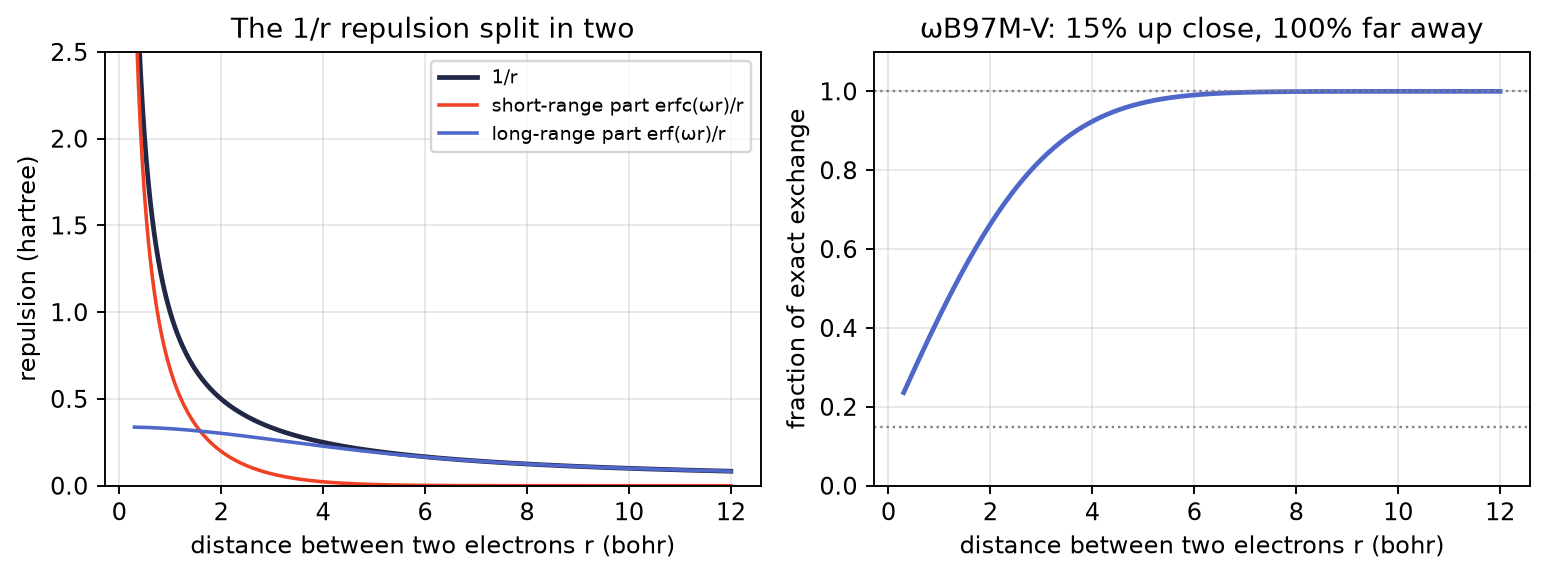
\includegraphics[width=0.85\linewidth]{figures/dft-range-split.png}
\caption{The short- and long-range parts of $1/r$ and the exact-exchange fractions of $\omega$B97M-V.}
\end{figure}

\begin{figure}[H]
\centering
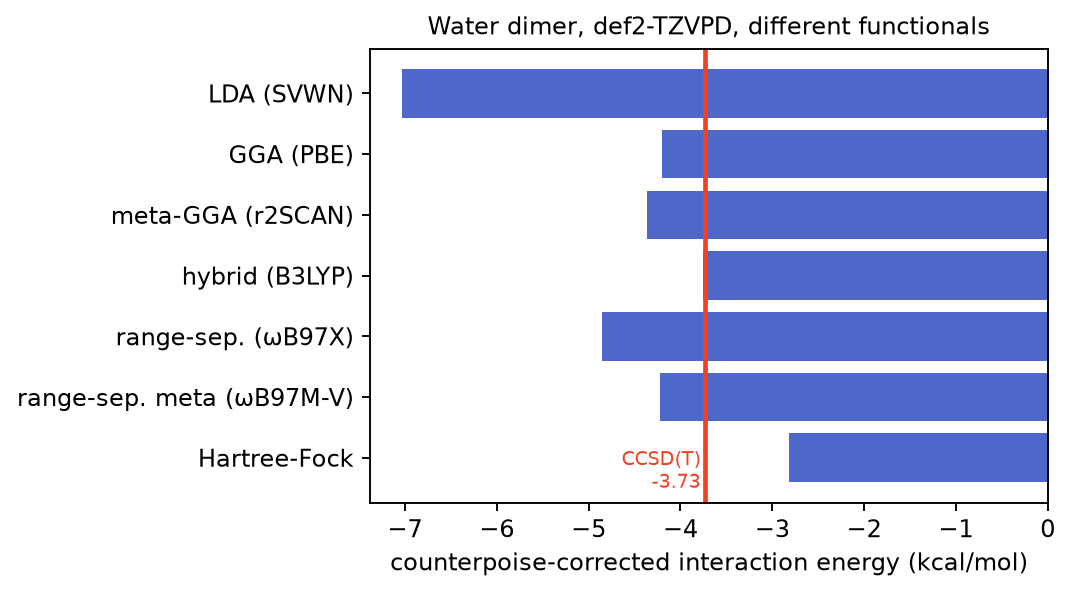
\includegraphics[width=0.85\linewidth]{figures/dft-water-dimer.png}
\caption{Water dimer interaction energy (counterpoise corrected, \texttt{def2-TZVPD}) for several methods, against coupled cluster in the same basis.}
\end{figure}

The reference is itself limited by the basis, so the bars are a comparison, not a ranking of truth. Local functionals over-bind the hydrogen bond, Hartree--Fock under-binds it, B3LYP lands closest (partly through cancelling errors, since it has no dispersion term), and $\omega$B97M-V binds about 0.5~kcal/mol more than the reference.

\subsection{Dispersion: -V against D3(BJ)}

London dispersion is an attraction between instantaneous fluctuations of the electron clouds of two molecules, falling as $-C_6/r^6$. It is \emph{non-local}: it connects density in one place with density in another, so local functionals and hybrid exchange cannot produce it. Two remedies are the difference between the two labels:
\begin{itemize}
\item \textbf{-V (VV10)} adds a non-local correlation term computed from the density on the grid; the functional's parameters were fitted together with it, so it is part of $\omega$B97M-V.
\item \textbf{-D3(BJ)} adds an empirical pairwise term $-\sum C_6/r^6+\cdots$ after the electronic calculation, with tabulated $C_6$ coefficients; the Becke--Johnson (BJ) damping function switches it off at short distance, where the functional already describes the electrons and the bare $-C_6/r^6$ would diverge.
\end{itemize}
The test is two methane molecules 3.8~\AA{} apart, which have no hydrogen bond or charge, so whatever binding they have is dispersion. Hartree--Fock and B3LYP find them repulsive; $\omega$B97M-V without VV10 leaves almost nothing; with VV10 the dimer binds by 0.42~kcal/mol, close to the coupled-cluster value 0.39.

\begin{figure}[H]
\centering
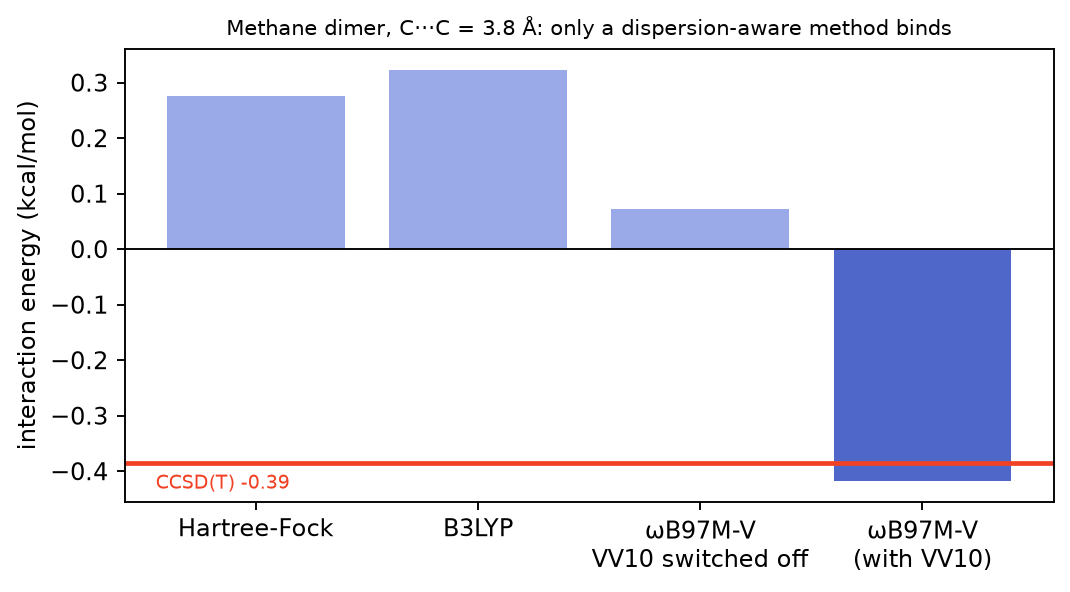
\includegraphics[width=0.85\linewidth]{figures/dft-methane-dimer.png}
\caption{Methane dimer at 3.8~\AA{}: interaction energy for several methods against coupled cluster.}
\end{figure}

\subsection{Settings that are not in the label}

DFT integrals of $E_{xc}$ are done numerically on a grid of points around each atom, specified as (radial, angular) points; the water calculations in these notes use $(99,590)$. Meta-GGAs and non-local terms are more sensitive to the grid than plain GGAs. The grid, the convergence criteria and the program (PySCF, ORCA, Psi4, Q-Chem) are not part of the label, so two groups with the ``same'' level of theory may differ by small amounts.

\paragraph{Further reading.} \cite{perdew,bursch,becke97,wb97x,wb97mv,vv10,d3,najibi,def2,grids,ecp,omol}.

%%%%%%%%%%%%%%%%%%%%%%%%%%%%%%%%%%%%%%%%%%%%%%%%%%%%%%%%%%%%%%%%%%%%%%%%%%%%%%%%%%%%%%%%%%%%%%%%%%%%%%%%%%%%%%%%%%%%%%%%%%%%%%%%%%%%
%% COUPLED CLUSTER
%%%%%%%%%%%%%%%%%%%%%%%%%%%%%%%%%%%%%%%%%%%%%%%%%%%%%%%%%%%%%%%%%%%%%%%%%%%%%%%%%%%%%%%%%%%%%%%%%%%%%%%%%%%%%%%%%%%%%%%%%%%%%%%%%%%%

\section{Coupled cluster: why CCSD(T) is the reference}\label{sec:cc}

\noindent\emph{Notebook: \texttt{coupled\_cluster.py}.}

\subsection{The exact answer, and why it is too expensive}

Hartree--Fock gives the best single determinant $\Phi_0$ of $N$ occupied spin orbitals and, in a basis of $M$ spatial orbitals, also $2M-N$ virtual ones. Every way of moving electrons from occupied to virtual orbitals gives another determinant: $\Phi_i^a$ (one electron moved, a single), $\Phi_{ij}^{ab}$ (two, a double), and so on. Together they span every antisymmetric wave function in the basis, and the exact answer in that basis is a combination of all of them,
\[
\Psi_{\text{FCI}}=c_0\Phi_0+\sum c_i^a\Phi_i^a+\sum c_{ij}^{ab}\Phi_{ij}^{ab}+\sum c_{ijk}^{abc}\Phi_{ijk}^{abc}+\cdots ,
\]
found by diagonalising the Hamiltonian between all determinants (full configuration interaction, FCI). The correlation energy in the basis is $E_{\text{FCI}}-E_{\text{HF}}$. The number of determinants is $\binom{M}{N_\alpha}\binom{M}{N_\beta}$, which grows exponentially: for water ($N_\alpha=N_\beta=5$) it is 1.7 million in the 6-31G basis, about $10^9$ in cc-pVDZ and about $10^{13}$ in cc-pVTZ. For water in the smallest basis, where FCI is feasible, the reference determinant carries most of the wave function and the doubles almost all of the remainder; singles, triples and quadruples together are a small fraction. So most of the exact answer is the reference plus pairs of electrons moved together.

\begin{figure}[H]
\centering
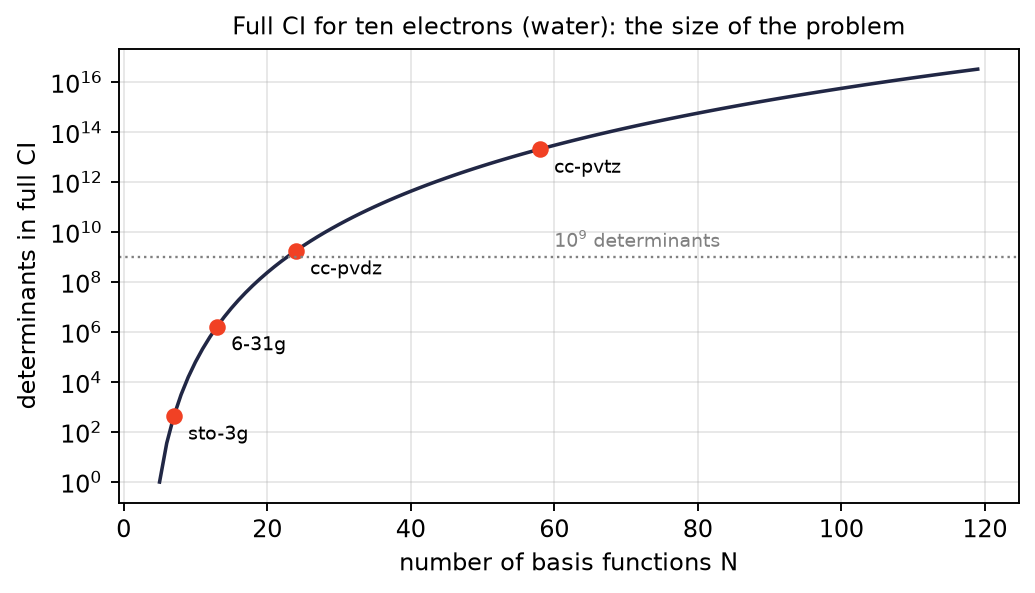
\includegraphics[width=0.8\linewidth]{figures/cc-determinants.png}
\caption{Number of determinants in FCI for water, by basis set.}
\end{figure}

\subsection{Truncating the exact answer breaks size consistency}

The obvious cut keeps determinants up to doubles: CISD, with coefficients from the lowest eigenvector of the Hamiltonian in that smaller space. It is variational and cheap, but it is not \emph{size consistent}: the energy of two molecules infinitely far apart should equal the sum of the energies of each alone, because an interaction energy is $E(AB)-E(A)-E(B)$ and the method must give zero when the molecules do not interact. For two distant molecules $A$ and $B$ the exact wave function contains ``a double on $A$ and a double on $B$ at once'', which from the pair is a quadruple excitation that CISD does not contain, so correlation in $A$ is squeezed out by correlation in $B$. The test with two non-interacting H$_2$ molecules shows that the Hartree--Fock energy of the pair is exactly twice that of one, and MP2, CCSD and FCI are additive, but CISD is not.

\begin{figure}[H]
\centering
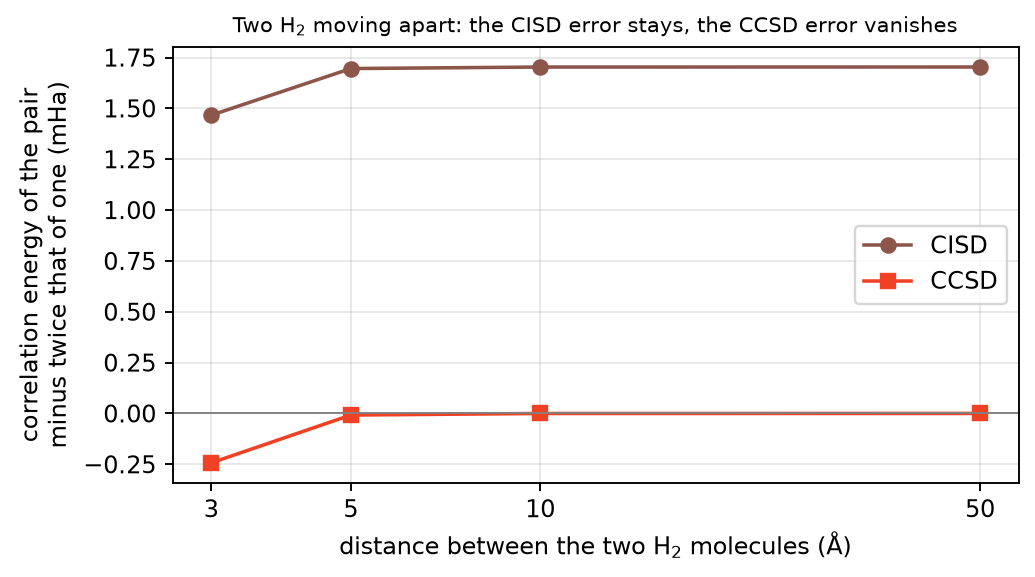
\includegraphics[width=0.85\linewidth]{figures/cc-size-consistency.png}
\caption{Two H$_2$ molecules at growing separation: correlation energy of the pair minus twice that of one. CCSD tends to zero; CISD levels off at a positive value.}
\end{figure}

\subsection{An exponential of excitations}

When $A$ and $B$ do not interact the wave function must be a product, $\Psi_{AB}=\Psi_A\Psi_B$, and the exponential is the function that turns sums into products. Let $a_p^\dagger$ put an electron into spin orbital $p$ and $a_p$ remove one. The operators for all single and double excitations, with amplitudes $t_i^a$ and $t_{ij}^{ab}$, are
\[
\hat T_1=\sum_{ia}t_i^a\,a_a^\dagger a_i,\qquad
\hat T_2=\frac14\sum_{ijab}t_{ij}^{ab}\,a_a^\dagger a_b^\dagger a_ja_i,\qquad
\hat T=\hat T_1+\hat T_2+\hat T_3+\cdots,
\]
and the coupled-cluster wave function is
\[
\Psi_{\text{CC}}=e^{\hat T}\Phi_0=\Big(1+\hat T+\tfrac12\hat T^2+\tfrac1{3!}\hat T^3+\cdots\Big)\Phi_0 .
\]
Keeping only $\hat T=\hat T_1+\hat T_2$ is \textbf{CCSD}. Because the excitation operators commute, the exponential can be expanded like numbers: the doubles come from $\hat T_2+\frac12\hat T_1^2$, the triples from $\hat T_1\hat T_2+\frac16\hat T_1^3$, the quadruples from $\frac12\hat T_2^2+\cdots$. So CCSD has the same number of unknowns as CISD, yet its wave function reaches determinants with any number of excitations: the higher ones are \emph{products} of the singles and doubles amplitudes (two pairs excited independently). What CCSD leaves out are the \emph{connected} triples, quadruples and higher, which have their own amplitudes. And \emph{size consistency is automatic}: for non-interacting $A$ and $B$, $\hat T=\hat T_A+\hat T_B$ with commuting parts, so
\[
e^{\hat T}\Phi_0=\big(e^{\hat T_A}\Phi_A\big)\big(e^{\hat T_B}\Phi_B\big),
\]
a product whose energy is the sum, and truncation at singles and doubles survives this. In the exact wave function of two independent H$_2$ molecules, the coefficient of the determinant with both molecules doubly excited equals the product of the two single-molecule double coefficients to six digits: this is the $\frac12\hat T_2^2$ term at work.

\subsection{The (T) correction}

The connected triples are left out of CCSD (the largest correction left at the usual single-reference level, from memory). Solving for them properly (CCSDT) is much more expensive, so the standard compromise is \textbf{CCSD(T)}: solve CCSD, then estimate the connected triples by perturbation theory once, from the converged amplitudes. In words, a triple excitation is reached from a double by exciting one more electron through the integrals; the energy is the square of that amplitude divided by an orbital-energy denominator, plus a cross term with the disconnected part built from the singles. The correction is computed once at the end, not iterated. CCSD costs about $N^6$ and CCSD(T) about $N^7$ in the size $N$ of the system (from memory), against $N^3$ to $N^4$ for DFT, which is why the method is used as the reference for small systems and not for production.

\paragraph{In four lines.} (1) Hartree--Fock misses the correlation energy, and the exact answer needs every excitation from $\Phi_0$ at a cost that grows exponentially. (2) Truncating the excitations (CISD) is not size consistent; writing the wave function as $e^{\hat T}\Phi_0$ with $\hat T=\hat T_1+\hat T_2$ is. (3) The amplitudes follow from projecting $e^{-\hat T}\hat He^{\hat T}\Phi_0=E\Phi_0$, and the series ends at fourth order (from memory). (4) CCSD(T) is the reference for the dimers above, where dispersion is a correlation effect that Hartree--Fock cannot give.

\paragraph{Further reading.} \cite{cc,triples,psi4np,crawfordcode,cbs}.

%%%%%%%%%%%%%%%%%%%%%%%%%%%%%%%%%%%%%%%%%%%%%%%%%%%%%%%%%%%%%%%%%%%%%%%%%%%%%%%%%%%%%%%%%%%%%%%%%%%%%%%%%%%%%%%%%%%%%%%%%%%%%%%%%%%%
%% TECHNICAL
%%%%%%%%%%%%%%%%%%%%%%%%%%%%%%%%%%%%%%%%%%%%%%%%%%%%%%%%%%%%%%%%%%%%%%%%%%%%%%%%%%%%%%%%%%%%%%%%%%%%%%%%%%%%%%%%%%%%%%%%%%%%%%%%%%%%

\section{Technical notes}

\subsection{Orbitals and basis functions are different things}

In $\psi_i=\sum_\mu C_{\mu i}\phi_\mu$ the basis functions $\phi_\mu$ are fixed ingredients and each orbital is a recipe that mixes them; the coefficients $C_{\mu i}$ connect the two sets of indices. The orbitals are orthonormal, $\int\psi_i\psi_j\,d\mathbf r=\delta_{ij}$, which in matrix form reads $\mathbf C^T\mathbf S\mathbf C=\mathbf 1$, while the basis functions overlap, so $\mathbf S\ne\mathbf 1$. If the $\phi_\mu$ were the true orbitals, $\mathbf S$ would be the identity and $\mathbf F$ diagonal, and there would be nothing to solve; the two meet in $\mathbf C^T\mathbf F\mathbf C=\boldsymbol\varepsilon$. The program's labels for basis functions (\texttt{O 1s}, \texttt{O 2px}) say only what shape a function has: the oxygen core orbital is not simply the basis function called \texttt{O 1s} but a mixture of several $s$-type functions of different spread.

\subsection{Why the hydrogen $\ell$-degeneracy is special}

The energy $-1/2n^2$ depends on $n$ only because the potential is exactly $-1/r$. In a many-electron atom the potential seen by one electron is $-Z_{\text{eff}}(r)/r$ with $Z_{\text{eff}}$ decreasing outward (section \ref{sec:hf}), which splits $s$, $p$ and $d$; and for the oscillator or the drumhead the ladder is different again. The shapes (the angular parts) survive in every spherically symmetric problem; the degeneracy in $\ell$ does not.

\subsection{What was checked, and what was not}

Every number below was computed in the notebooks of the \texttt{qm-theory} repository, whose test suites run as \texttt{pytest} checks.

\paragraph{Checked numerically.}
\begin{itemize}
\item \emph{Boxes and hydrogen:} the box energies and node counts, the degeneracies of the square and cube, the orthonormality of the spherical harmonics and of whole orbitals, $\ell(\ell+1)$ by finite differences, the radial energies against $-1/2n^2$, the degeneracy $n^2$, and that the nodes of orbitals lie on the stated spheres, cones and planes.
\item \emph{Bridge:} the H$_2^+$ curve (minimum at $R\approx2.0$ bohr; harmonic wavenumber $2312\ \text{cm}^{-1}$ and level spacing $2189\ \text{cm}^{-1}$ from the nuclear problem), the hybrid angles and orthonormality (also by integration over the sphere), the methane toy levels against its $2\times2$ blocks, and that the four bond orbitals span the occupied space exactly.
\item \emph{Hartree--Fock:} the helium minimum $\zeta=1.6875$ with $E=-2.84766$; the closed form of $v_J(r)$ and the identity $\int\lvert\varphi\rvert^2v_J\,d\mathbf r=\frac58\zeta$ by numerical integration; $Z_{\text{eff}}(r)$ of lithium; $s<p<d$ in the screened toy; the helium orbital energy.
\item \emph{Basis sets:} the H$_2^+$ two-function integrals against quadrature, the STO-3G and STO-6G coefficients against PySCF, the Gaussian product theorem, the shell sizes and the water basis-function counts.
\item \emph{DFT:} the water SCF and the $\omega$B97M-V exchange fractions (from PySCF; the matrix elements of $\mathbf F$ are stored with the data), and the methane and water dimer interaction energies (stored PySCF runs).
\item \emph{Coupled cluster:} a numpy implementation of CISD, CCSD and (T) agrees with PySCF to better than $10^{-8}$ hartree on H$_2$ and water; the size-consistency test on two H$_2$ molecules.
\end{itemize}

\paragraph{Not checked here, or stated from memory.}
\begin{itemize}
\item The helium exact and Hartree--Fock-limit energies ($-2.9037$, $-2.8617$ hartree) and the real methane numbers (orbital energies, the $20/76/4$ composition) are literature or stored values, not recomputed here.
\item The cost exponents of HF, DFT, CCSD and CCSD(T), that the series of equations ends at fourth order, that the connected triples are the largest correction left after CCSD, and that CCSD(T) reaches a fraction of a kcal/mol for interaction energies in large basis sets are from memory.
\item The toy models (screening with one free core size, methane) use invented parameters and show only the ordering and the pattern of levels.
\item The CCSD(T) reference for the dimers is in one basis (\texttt{def2-TZVPD}) and is not extrapolated to the complete-basis limit.
\item The functional and basis-set citations (Becke 97, $\omega$B97X, $\omega$B97M-V, VV10, D3, D3(BJ), \texttt{def2}, and others in the bibliography) were checked on 13 November 2026 for title, authors, year, journal, volume and pages against the Crossref record of the DOI; the papers themselves were not read. Open: whether Najibi and Goerigk (2018) defines $\omega$B97M-D3(BJ).
\end{itemize}


\begin{thebibliography}{99}
\bibitem{lt35} LibreTexts, \emph{Physical Chemistry}, 3.5, ``The energy of a particle in a box is quantized''. \url{https://chem.libretexts.org/Bookshelves/Physical_and_Theoretical_Chemistry_Textbook_Maps/Physical_Chemistry_(LibreTexts)/03:_The_Schrodinger_Equation_and_a_Particle_in_a_Box/3.05:_The_Energy_of_a_Particle_in_a_Box_is_Quantized}

\bibitem{lt39} LibreTexts, \emph{Physical Chemistry}, 3.9, ``A particle in a three-dimensional box''. \url{https://chem.libretexts.org/Bookshelves/Physical_and_Theoretical_Chemistry_Textbook_Maps/Physical_Chemistry_(LibreTexts)/03:_The_Schrodinger_Equation_and_a_Particle_in_a_Box/3.09:_A_Particle_in_a_Three-Dimensional_Box}

\bibitem{uc73} Physics LibreTexts (UC Davis, Physics 9HC), 7.3, ``Central forces''. \url{https://phys.libretexts.org/Courses/University_of_California_Davis/UCD:_Physics_9HC__Introduction_to_Waves_Physical_Optics_and_Quantum_Theory/7:_Quantum_Theory_in_Three_Dimensions/7.3:_Central_Forces}

\bibitem{puc62} LibreTexts (Pacific Union College, \emph{Quantum Chemistry}), 6.2, ``The wavefunctions of a rigid rotator are called spherical harmonics''. \url{https://chem.libretexts.org/Courses/Pacific_Union_College/Quantum_Chemistry/06:_The_Hydrogen_Atom/6.02:_The_Wavefunctions_of_a_Rigid_Rotator_are_Called_Spherical_Harmonics}

\bibitem{puc64} LibreTexts (Pacific Union College), 6.4, ``Hydrogen atomic orbitals depend upon three quantum numbers''. \url{https://chem.libretexts.org/Courses/Pacific_Union_College/Quantum_Chemistry/06\%3A_The_Hydrogen_Atom/6.04\%3A_Hydrogen_Atomic_Orbitals_Depend_upon_Three_Quantum_Numbers}

\bibitem{fowler} Physics LibreTexts (Fowler, \emph{Quantum Mechanics}), 4.6, ``The hydrogen atom''. \url{https://phys.libretexts.org/Bookshelves/Quantum_Mechanics/Quantum_Mechanics_(Fowler)/04:_Angular_Momentum_Spin_and_the_Hydrogen_Atom/4.06:_The_Hydrogen_Atom}

\bibitem{grinnell} LibreTexts (Grinnell College, CHM 364), 6.6, ``Orbital angular momentum and the p-orbitals'' (real and complex orbitals). \url{https://chem.libretexts.org/Courses/Grinnell_College/CHM_364:_Physical_Chemistry_2_(Grinnell_College)/06:_The_Hydrogen_Atom/6.06:_Orbital_Angular_Momentum_and_the_p-Orbitals}

\bibitem{lt92} LibreTexts, \emph{Physical Chemistry}, 9.2, ``The H$_2^+$ prototypical species'' (Born--Oppenheimer, LCAO). \url{https://chem.libretexts.org/Bookshelves/Physical_and_Theoretical_Chemistry_Textbook_Maps/Physical_Chemistry_(LibreTexts)/09\%3A_Chemical_Bonding_in_Diatomic_Molecules/9.02\%3A_The_H_Prototypical_Species}

\bibitem{puc8} LibreTexts (Pacific Union College), chapter 8, ``Multielectron atoms'': 8.2 helium and the variational method, 8.3 the self-consistent field method, 8.6 Slater determinants. \url{https://chem.libretexts.org/Courses/Pacific_Union_College/Quantum_Chemistry/08\%3A_Multielectron_Atoms}

\bibitem{morsch} LibreTexts, \emph{Organic Chemistry} (Morsch et al.), 1.6, ``sp$^3$ hybrid orbitals and the structure of methane''. \url{https://chem.libretexts.org/Bookshelves/Organic_Chemistry/Organic_Chemistry_(Morsch_et_al.)/01:_Structure_and_Bonding/1.06:_sp_Hybrid_Orbitals_and_the_Structure_of_Methane}

\bibitem{rioux} LibreTexts, Rioux, \emph{Quantum Tutorials}, 3.18, ``A molecular orbital approach to bonding in methane''. \url{https://chem.libretexts.org/Bookshelves/Physical_and_Theoretical_Chemistry_Textbook_Maps/Quantum_Tutorials_(Rioux)/03:_Chemical_Bonding/3.18:_A_Molecular_Orbital_Approach_to_Bonding_in_Methane}

\bibitem{sherrillnotes} C. D. Sherrill, ``An introduction to Hartree--Fock molecular orbital theory'', Georgia Institute of Technology, June 2000 (8 pages; read in full on 13 November 2026; the order of section \ref{sec:hf} follows it). \url{https://vergil.chemistry.gatech.edu/static/content/hf-intro.pdf}

\bibitem{sherrillbasis} C. D. Sherrill, ``Basis sets in quantum chemistry'' (lecture slides), Georgia Institute of Technology. \url{https://vergil.chemistry.gatech.edu/basis-sets.pdf}

\bibitem{hehre} W. J. Hehre, R. F. Stewart and J. A. Pople, J. Chem. Phys. \textbf{51}, 2657 (1969). \href{https://doi.org/10.1063/1.1672392}{doi:10.1063/1.1672392}

\bibitem{bse} Basis Set Exchange, \url{https://www.basissetexchange.org/}; B. P. Pritchard et al., J. Chem. Inf. Model. \textbf{59}, 4814 (2019), \href{https://doi.org/10.1021/acs.jcim.9b00725}{doi:10.1021/acs.jcim.9b00725}

\bibitem{def2} F. Weigend and R. Ahlrichs, Phys. Chem. Chem. Phys. \textbf{7}, 3297 (2005), \href{https://doi.org/10.1039/b508541a}{doi:10.1039/b508541a}; D. Rappoport and F. Furche, J. Chem. Phys. \textbf{133}, 134105 (2010), \href{https://doi.org/10.1063/1.3484283}{doi:10.1063/1.3484283}

\bibitem{bsse} S. F. Boys and F. Bernardi, Mol. Phys. \textbf{19}, 553 (1970), \href{https://doi.org/10.1080/00268977000101561}{doi:10.1080/00268977000101561}

\bibitem{kohn} W. Kohn and L. J. Sham, Phys. Rev. \textbf{140}, A1133 (1965), \href{https://doi.org/10.1103/PhysRev.140.A1133}{doi:10.1103/PhysRev.140.A1133}

\bibitem{burke} K. Burke, \emph{The ABC of DFT} (free draft), \url{https://dft.uci.edu/learnDFT.php}; J. Toulouse, ``Review of approximations for the exchange-correlation energy in density-functional theory'', \href{https://arxiv.org/abs/2103.02645}{arXiv:2103.02645}

\bibitem{psi4np} Psi4NumPy tutorials (Hartree--Fock, density functional theory, CEPA0 and CCD), \url{https://github.com/psi4/psi4numpy/tree/master/Tutorials}

\bibitem{perdew} J. P. Perdew, AIP Conf. Proc. \textbf{577}, 1 (2001), \href{https://doi.org/10.1063/1.1390175}{doi:10.1063/1.1390175}

\bibitem{bursch} M. Bursch, J.-M. Mewes, A. Hansen and S. Grimme, Angew. Chem. Int. Ed. \textbf{61}, e202205735 (2022), \href{https://doi.org/10.1002/anie.202205735}{doi:10.1002/anie.202205735}; N. Mardirossian and M. Head-Gordon, Mol. Phys. \textbf{115}, 2315 (2017), \href{https://doi.org/10.1080/00268976.2017.1333644}{doi:10.1080/00268976.2017.1333644}

\bibitem{becke97} A. D. Becke, J. Chem. Phys. \textbf{107}, 8554 (1997), \href{https://doi.org/10.1063/1.475007}{doi:10.1063/1.475007}

\bibitem{wb97x} J.-D. Chai and M. Head-Gordon, J. Chem. Phys. \textbf{128}, 084106 (2008), \href{https://doi.org/10.1063/1.2834918}{doi:10.1063/1.2834918} ($\omega$B97X); Phys. Chem. Chem. Phys. \textbf{10}, 6615 (2008), \href{https://doi.org/10.1039/b810189b}{doi:10.1039/b810189b} ($\omega$B97X-D)

\bibitem{wb97mv} N. Mardirossian and M. Head-Gordon, J. Chem. Phys. \textbf{144}, 214110 (2016), \href{https://doi.org/10.1063/1.4952647}{doi:10.1063/1.4952647}

\bibitem{vv10} O. A. Vydrov and T. Van Voorhis, J. Chem. Phys. \textbf{133}, 244103 (2010), \href{https://doi.org/10.1063/1.3521275}{doi:10.1063/1.3521275}

\bibitem{d3} S. Grimme, J. Antony, S. Ehrlich and H. Krieg, J. Chem. Phys. \textbf{132}, 154104 (2010), \href{https://doi.org/10.1063/1.3382344}{doi:10.1063/1.3382344}; S. Grimme, S. Ehrlich and L. Goerigk, J. Comput. Chem. \textbf{32}, 1456 (2011), \href{https://doi.org/10.1002/jcc.21759}{doi:10.1002/jcc.21759} (D3(BJ))

\bibitem{najibi} A. Najibi and L. Goerigk, J. Chem. Theory Comput. \textbf{14}, 5725 (2018), \href{https://doi.org/10.1021/acs.jctc.8b00842}{doi:10.1021/acs.jctc.8b00842}

\bibitem{pyscfdft} PySCF documentation, ``Density functional theory (DFT)'' (integration grids) and ``Molecular structure'' (basis sets, ECPs), \url{https://pyscf.org/user/dft.html}, \url{https://pyscf.org/user/gto.html}

\bibitem{grids} R. Treutler and R. Ahlrichs, J. Chem. Phys. \textbf{102}, 346 (1995), \href{https://doi.org/10.1063/1.469408}{doi:10.1063/1.469408}; S. Dasgupta and J. M. Herbert, J. Comput. Chem. \textbf{38}, 869 (2017), \href{https://doi.org/10.1002/jcc.24761}{doi:10.1002/jcc.24761}

\bibitem{ecp} P. J. Hay and W. R. Wadt, J. Chem. Phys. \textbf{82}, 270 (1985), \href{https://doi.org/10.1063/1.448799}{doi:10.1063/1.448799}; M. Dolg and X. Cao, Chem. Rev. \textbf{112}, 403 (2012), \href{https://doi.org/10.1021/cr2001383}{doi:10.1021/cr2001383}

\bibitem{omol} D. S. Levine et al., ``The Open Molecules 2025 (OMol25) dataset, evaluations, and models'', \href{https://arxiv.org/abs/2505.08762}{arXiv:2505.08762}; P. Eastman et al., Sci. Data \textbf{10}, 11 (2023), \href{https://doi.org/10.1038/s41597-022-01882-6}{doi:10.1038/s41597-022-01882-6}

\bibitem{cc} T. D. Crawford and H. F. Schaefer, Rev. Comput. Chem. \textbf{14}, 33 (2000), \href{https://doi.org/10.1002/9780470125915.ch2}{doi:10.1002/9780470125915.ch2}; R. J. Bartlett and M. Musia{\l}, Rev. Mod. Phys. \textbf{79}, 291 (2007), \href{https://doi.org/10.1103/RevModPhys.79.291}{doi:10.1103/RevModPhys.79.291}

\bibitem{triples} K. Raghavachari, G. W. Trucks, J. A. Pople and M. Head-Gordon, Chem. Phys. Lett. \textbf{157}, 479 (1989), \href{https://doi.org/10.1016/S0009-2614(89)87395-6}{doi:10.1016/S0009-2614(89)87395-6}

\bibitem{cbs} T. Helgaker, W. Klopper, H. Koch and J. Noga, J. Chem. Phys. \textbf{106}, 9639 (1997), \href{https://doi.org/10.1063/1.473863}{doi:10.1063/1.473863}; Psi4 manual, \texttt{cbs()}, \url{https://psicode.org/psi4manual/master/api/psi4.driver.cbs.html}

\bibitem{crawfordcode} Crawford group, \emph{Programming Projects}, \url{https://github.com/CrawfordGroup/ProgrammingProjects}
\end{thebibliography}

\end{document}
